\subsection{测度的逆极限}

设 X、Y 是两个紧空间，\(p : X \to Y\) 是一个连续映射；则 \(f \mapsto f \circ p\) 是 \(\mathcal{C}(Y; \mathbf{C})\) 到 \(\mathcal{C}(X; \mathbf{C})\) 中的一个连续线性映射，因为 \(\|f \circ p\| \leqslant \|f\|\) 对每个函数 \(f \in \mathcal{C}(Y; \mathbf{C})\) 都成立；我们把这个映射记作 \(p'\) 。于是它的转置 \(^{t}p' : M(X; C) \to M(Y; C)\) 具有如下性质：对 X 上的每个测度 \(\mu\) ，\(^{t}p'(\mu)\) 是 Y 上满足

\[
\langle^ {t} p ^ {\prime} (\mu), f \rangle = \langle \mu , f \circ p \rangle
\]

对每个函数 \(f \in \mathcal{C}(\mathrm{Y};\mathbf{C})\) 都成立的测度。注意，对每个 \(x \in \mathrm{X}\) ，有 \(^t p'(\varepsilon_x) = \varepsilon_{p(x)}\) ；为此，我们用 \(p_*(\mu)\) 表示测度 \(^t p'(\mu)\) ，它就这样延拓了 \(p\) ，当 \(\mathrm{X}\) （相应地 \(\mathrm{Y}\) ）典范地嵌入 \(\mathcal{M}(\mathrm{X};\mathbf{C})\) （相应地 \(\mathcal{M}(\mathrm{Y};\mathbf{C})\) ）时（§1, No.~9, 命题 13）；对每个测度 \(\mu\) （\(\mathrm{X}\) 上的），\(p_*(\mu)\) 是测度的像这一一般概念（我们将在 Ch. V, §6 中研究）的特例。由于我们上面已经看到 \(\| p' \| \leqslant 1\) ，故也有 \(\| ^t p' \| \leqslant 1\) ，从而

\[
\| p _ {*} (\mu) \| \leqslant \| \mu \|\tag{15}
\]

对每个测度 \(\mu \in \mathcal{M}(\mathrm{X};\mathbf{C})\) 成立。

现在考虑一个有向预序集 I，以及一个逆系统（或称"射影系统"）\((\mathrm{X}_{\alpha}, p_{\alpha\beta})\) ，它由紧空间 \(X_{\alpha}\) （GT, I, §4, No.~4）组成，以 I 为指标集；已知逆极限空间 \(X = \varprojlim X_{\alpha}\) 是紧的（GT, I, §9, No.~6, 命题 8）；我们将用 \(p_{\alpha}\) 表示 X 到 \(X_{\alpha}\) 中的典范映射。

显然，\((\mathcal{M}(\mathrm{X}_{\alpha};\mathbf{C}),(p_{\alpha\beta})_{*})\) 是向量空间的一个逆系统，而 \(((p_{\alpha})_{*})\) 是线性映射的一个逆系统，这就为下述定义提供了依据：

定义 2. --- 设 \((\mu_{\alpha})_{\alpha \in I}\) 是一个族，其中对每个 \(\alpha \in I\) ，\(\mu_{\alpha}\) 是 \(X_{\alpha}\) 上的一个测度；若当 \(\alpha \leqslant \beta\) 时总有 \(\mu_{\alpha} = (p_{\alpha \beta})_{*}(\mu_{\beta})\) ，则称该族为测度的一个逆系统。测度 \(\mu\) （在 \(X = \varprojlim X_{\alpha}\) 上）称为逆系统 \((\mu_{\alpha})\) 的一个逆极限，如果 \(\mu_{\alpha} = (p_{\alpha})_{*}(\mu)\) 对每个 \(\alpha \in I\) 成立。

命题 8. --- （i）若测度逆系统 \((\mu_{\alpha})\) （在诸 \(X_{\alpha}\) 上）有逆极限，则该逆极限是唯一的。

\begin{enumerate}
\def\labelenumi{(\roman{enumi})}
\setcounter{enumi}{1}
\item
  若逆系统 \((\mu_{\alpha})\) 有逆极限，则范数族 \((\| \mu_{\alpha}\|)\) 有界。
\item
  若诸 \(p_{\alpha\beta}\) 都是满射且族 ( \(\|\mu_{\alpha}\|\) ) 有界，则测度逆系统 ( \(\mu_{\alpha}\) ) 有逆极限。
\item
  若诸 \(p_{\alpha \beta}\) 都是满射，则每个正测度逆系统 \((\mu_{\alpha})\) 都有一个逆极限 \(\mu\) ，它是 \(X\) 上的正测度，且 \(\| \mu \| = \| \mu_{\alpha} \|\) 对所有 \(\alpha\) 成立。
\end{enumerate}

\begin{enumerate}
\def\labelenumi{(\roman{enumi})}
\tightlist
\item
  我们首先证明下述引理：
\end{enumerate}

引理 3. --- 设 F 是由具有下述性质的函数 \(f \in \mathcal{C}(\mathrm{X};\mathbf{C})\) 所成的集：存在 \(\alpha \in \mathrm{I}\) 和函数 \(f_{\alpha} \in \mathcal{C}(\mathrm{X}_{\alpha};\mathbf{C})\) 使 \(f = f_{\alpha} \circ p_{\alpha}\) 。则 F 是 \(\mathcal{C}(\mathrm{X};\mathbf{C})\) 的一个稠密线性子空间。

我们首先注意，若 \(g = g_{\beta} \circ p_{\beta}\) 且 \(h = h_{\gamma} \circ p_{\gamma}\) ，其中 \(g_{\beta} \in \mathcal{C}(\mathrm{X}_{\beta}; \mathbf{C})\) ，\(h_{\gamma} \in \mathcal{C}(\mathrm{X}_{\gamma}; \mathbf{C})\) ，则存在 \(\alpha \in I\) 使 \(\alpha \geqslant \beta\) 且 \(\alpha \geqslant \gamma\) ，于是 \(p_{\beta} = p_{\beta\alpha} \circ p_{\alpha}\) ，\(p_{\gamma} = p_{\gamma\alpha} \circ p_{\alpha}\) ，由此可知

\[
g + h = \left(g _ {\beta} \circ p _ {\beta \alpha} + h _ {\gamma} \circ p _ {\gamma \alpha}\right) \circ p _ {\alpha}
\]

属于 F；同理可见 \(gh \in F\) ；于是 F 是 \(\mathcal{C}(\mathrm{X};\mathbf{C})\) 的一个 C-子代数，它包含常数，并且关系 \(f \in F\) 蕴涵 \(\overline{f} \in F\) 。最后，若 \(x \neq y\) 是 X 的两个点，则存在 \(\alpha \in I\) 使 \(p_{\alpha}(x) \neq p_{\alpha}(y)\) ，因而存在函数 \(f_{\alpha} \in \mathcal{C}(\mathrm{X}_{\alpha};\mathbf{C})\) 使 \(f_{\alpha}(p_{\alpha}(x)) \neq f_{\alpha}(p_{\alpha}(y))\) 。于是结论由 Stone--Weierstrass 定理（GT, X, §4, No.~4, 命题 7）得出。

引理既已建立，设 \(\mu, \mu'\) 是 X 上两个使 \((p_{\alpha})_{*}(\mu) = (p_{\alpha})_{*}(\mu')\) 对所有 \(\alpha \in I\) 成立的测度；这就是说，对每个 \(\alpha \in I\) 和每个函数 \(f_{\alpha} \in \mathcal{C}(X_{\alpha}; \mathbf{C})\) ，有

\[
\left\langle f _ {\alpha}, \left(p _ {\alpha}\right) _ {*} (\mu) \right\rangle = \left\langle f _ {\alpha}, \left(p _ {\alpha}\right) _ {*} \left(\mu^ {\prime}\right) \right\rangle ,
\]

即 \(\langle f_{\alpha} \circ p_{\alpha}, \mu \rangle = \langle f_{\alpha} \circ p_{\alpha}, \mu' \rangle\) ；换句话说，\(\mu\) 与 \(\mu'\) 在 \(\mathcal{C}(\mathrm{X}; \mathbf{C})\) 的子空间 F 上一致，而由引理 3，F 是稠密的，因此 \(\mu = \mu'\) ，这就证明了（i）。

\begin{enumerate}
\def\labelenumi{(\roman{enumi})}
\setcounter{enumi}{1}
\tightlist
\item
  把关系式 (15) 应用于 \(p_{\alpha}\) 就表明：若 \(\mu\) 是逆系统 \((\mu_{\alpha})\) 的逆极限，则必有
\end{enumerate}

\[
\| \mu \| \geqslant \| \mu_ {\alpha} \|\tag{16}
\]

对所有 \(\alpha \in I\) 成立。

\begin{enumerate}
\def\labelenumi{(\roman{enumi})}
\setcounter{enumi}{2}
\tightlist
\item
  设诸 \(p_{\alpha \beta}\) 都是满射；已知诸 \(p_{\alpha}\) 此时也都是满射（GT, I, §9, No.~6, 命题 8）。考虑一个测度逆系统 \((\mu_{\alpha})\) ，我们先证明在 F 上（沿用引理 3 的记号）存在一个线性形式 \(\lambda\) ，使得对每个 \(\alpha \in \mathbf{I}\) 和每个 \(f_{\alpha} \in \mathcal{C}(\mathrm{X}_{\alpha}; \mathbf{C})\) ，有 \(\lambda(f_{\alpha} \circ p_{\alpha}) = \mu_{\alpha}(f_{\alpha})\) 。为此，设 \(\beta, \gamma\) 是 I 中两个指标，且 \(f_{\beta} \in \mathcal{C}(\mathrm{X}_{\beta}; \mathbf{C})\) 与 \(f_{\gamma} \in \mathcal{C}(\mathrm{X}_{\gamma}; \mathbf{C})\) 是满足 \(f_{\beta} \circ p_{\beta} = f_{\gamma} \circ p_{\gamma}\) 的两个函数；则存在指标 \(\alpha \in \mathbf{I}\) 使 \(\alpha \geqslant \beta\) 且 \(\alpha \geqslant \gamma\) ，因此
\end{enumerate}

\[
p _ {\beta} = p _ {\beta \alpha} \circ p _ {\alpha}, p _ {\gamma} = p _ {\gamma \alpha} \circ p _ {\alpha} \quad \text {and} \quad (f _ {\beta} \circ p _ {\beta \alpha}) \circ p _ {\alpha} = (f _ {\gamma} \circ p _ {\gamma \alpha}) \circ p _ {\alpha};
\]

由于 \(p_{\alpha}\) 是满射，这就蕴涵 \(f_{\beta} \circ p_{\beta \alpha} = f_{\gamma} \circ p_{\gamma \alpha}\) ，因此

\[
\mu_ {\alpha} (f _ {\beta} \circ p _ {\beta \alpha}) = \mu_ {\alpha} (f _ {\gamma} \circ p _ {\gamma \alpha});
\]

但按定义，最后这个关系也可写成 \(\mu_{\beta}(f_{\beta}) = \mu_{\gamma}(f_{\gamma})\) ，即得我们的断言。

在此条件下，假设存在一个有限数 \(a > 0\) 使 \(\| \mu_{\alpha}\| \leqslant a\) 对所有 \(\alpha \in \mathrm{I}\) 成立；则对每个函数 \(f_{\alpha} \in \mathcal{C}(\mathrm{X}_{\alpha};\mathbf{C})\) ，

\[
\left| \lambda (f _ {\alpha} \circ p _ {\alpha}) \right| = \left| \mu_ {\alpha} (f _ {\alpha}) \right| \leqslant a \| f _ {\alpha} \| = a \| f _ {\alpha} \circ p _ {\alpha} \|
\]

这是因为 \(p_{\alpha}\) 是满射。这表明线性形式 \(\lambda\) 在 \(\mathbf{F}\) 上连续，且由引理 3 可知，\(\lambda\) 可以延拓为测度 \(\mu\) （\(\mathbf{X}\) 上的），使 \((p_{\alpha})_{*}(\mu) = \mu_{\alpha}\) 对所有 \(\alpha \in \mathbf{I}\) 成立，这就证明了（iii）。

\begin{enumerate}
\def\labelenumi{(\roman{enumi})}
\setcounter{enumi}{3}
\tightlist
\item
  为证明 \(\mu\) 的存在性，由（iii）只需验证范数族 ( \(\| \mu_{\alpha}\|\) ) 有界。但 \(\| \mu_{\alpha}\| = \mu_{\alpha}(1)\) ，且当 \(\alpha \leqslant \beta\) 时，关系 \(\mu_{\alpha} = (p_{\alpha \beta})_{*}(\mu_{\beta})\) 蕴涵 \(\mu_{\alpha}(1) = \mu_{\beta}(1)\) ；由于 I 是有向的，所有测度 \(\mu_{\alpha}\) 的总质量因此都相等，即得我们的断言。此外，子空间 F 显然满足 §1, No.~7, 命题 9 中的性质（P），因此逆极限测度 \(\mu\) （\((\mu_{\alpha})\) 的）是正测度。最后，关系 \(\mu_{\alpha} = (p_{\alpha})_{*}(\mu)\) 如上一样表明 \(\mu(1) = \mu_{\alpha}(1)\) 。
\end{enumerate}

例子. --- 设 \((\mathrm{X}_{\lambda})_{\lambda\in\mathrm{L}}\) 是紧空间的一个族；令 \(X=\prod_{\lambda\in L}X_{\lambda}\) ，且对 L 的每个有限子集 J，令 \(X_{J}=\prod_{\lambda\in J}X_{\lambda}\) ；用 \(pr_{J}:X\to X_{J}\) 与 \(pr_{J,K}:X_{K}\to X_{J}\) （对 \(J\subset K\) ）表示典范投影。我们知道 \((\mathrm{X}_{\mathrm{J}},\mathrm{pr}_{\mathrm{JK}})\) 是紧空间的一个逆系统，且连续映射系统 \((\mathrm{pr}_{\mathrm{J}})\) 的逆极限是 X 到逆极限空间 \(\varprojlim X_{J}\) 上的一个同胚，从而可以把这两个空间等同起来（GT, I, §4, No.~4 及 S, III, §7, No.~2, 注 3）。由于诸投影 \(pr_{J,K}\) 是满射，故由命题 8 可知，集合 \(\mathcal{M}(\mathrm{X};\mathbf{C})\) （相应地 \(\mathcal{M}_{+}(\mathrm{X})\) ）可以等同于逆系统 \((\mu_{\mathrm{J}})\) 中使范数族 \((\|\mu_{\mathrm{J}}\|)\) 有界的那些所成的集（相应地，使诸 \(\mu_{J}\) 全为正测度、从而总质量必然相同的那些所成的集）。

我们特别考虑这样的情形：对每个 \(\lambda \in L\) ，给定测度 \(\mu_{\lambda}\) 于 \(X_{\lambda}\) 上，并令 \(\mu_{J} = \bigotimes_{\lambda \in J} \mu_{\lambda}\) 。若 \(J \subset K\) 是 I 的两个有限子集，则对每个函数 \(f_{J} \in \mathcal{C}(X_{J}; \mathbf{C})\) ，依据 No.~4 的公式 (14)，有

\[
\mu_ {K} \left(f _ {J} \circ \operatorname{pr} _ {J, K}\right) = \mu_ {J} \left(f _ {J}\right) \cdot \prod_ {\lambda \in K - J} \mu_ {\lambda} (1).\tag{17}
\]

因此，为使 \((\mu_{\mathrm{J}})\) 是测度逆系统，必须且只须：或者 \(\mu_{\lambda}=0\) 对所有 \(\lambda\in L\) 成立，或者 \(\mu_{\lambda}(1)=1\) 对所有 \(\lambda\in L\) 成立。

\subsection{测度的无穷乘积}

设 \((\mathbf{X}_{\lambda})_{\lambda \in \mathbf{L}}\) 是紧空间的一个族，且对每个 \(\lambda \in \mathbf{L}\) ，设 \(\mu_{\lambda}\) 是 \(\mathbf{X}_{\lambda}\) 上的一个测度。我们沿用 No.~5 例子中的记号，于是特别地，\(\mu_{\mathrm{J}} = \bigotimes_{\lambda \in \mathrm{J}} \mu_{\lambda}\) 对每个有限子集 \(J\) ⊂ \(L\) 成立。

命题 9. --- 假设诸测度 \(\mu_{\lambda}\) 都是正测度，且族 \((\mu_{\lambda}(1))_{\lambda \in L}\) 在 \(\mathbf{R}_{+}\) 中可乘（乘积可能为 0）。则存在唯一的测度 \(\mu\) 于 X 上，使得对 L 的每个有限子集 J 和每个函数 \(f_{J} \in \mathcal{C}(X_J; C)\) ，

\[
\mu (f _ {\mathrm{J}} \circ \mathrm{pr} _ {\mathrm{J}}) = \mu_ {\mathrm{J}} (f _ {\mathrm{J}}) \prod_ {\lambda \in \mathrm{L} - \mathrm{J}} \mu_ {\lambda} (1).\tag{18}
\]

此外，测度 \(\mu\) 是正测度，其总质量由

\[
\mu (1) = \prod_ {\lambda \in L} \mu_ {\lambda} (1).\tag{19}
\]

设 \(\mathbf{F}\) 是由 \(\mathbf{X}\) 上形如 \(f_{\mathrm{J}} \circ \mathrm{pr}_{\mathrm{J}}\) 的函数所构成的向量空间，其中 \(\mathbf{J}\) 取遍 \(\mathbf{L}\) 的有限子集组成的有向集，而 \(f_{\mathrm{J}} \in \mathcal{C}(\mathrm{X}_{\mathrm{J}}; \mathbf{C})\) ；我们也把 \(\mathbf{F}\) 称为 \(\mathbf{X}\) 上只依赖于有限个变量的连续函数所成的空间。No.~5 的引理 3 表明 \(\mathbf{F}\) 在 \(\mathcal{C}(\mathrm{X}; \mathbf{C})\) 中稠密，这就证明了唯一性断言。 若 \(\mu_{\lambda_0} = 0\) 对某个 \(\lambda_0 \in \mathbf{L}\) 成立，则测度 \(\mu = 0\) 即满足要求，因为在 (18) 的右端中，\(\mu_{\mathrm{J}}(f_{\mathrm{J}}) = 0\) 当 \(\lambda_0 \in \mathbf{J}\) 时成立，而 \(\prod_{\lambda \in \mathbf{L} - \mathbf{J}} \mu_{\lambda}(1) = 0\) 当 \(\lambda_0 \notin \mathbf{J}\) 时成立。于是可以假设 \(\mu_{\lambda} \neq 0\) 对所有 \(\lambda \in \mathbf{J}\) 成立，又因诸测度 \(\mu_{\lambda}\) 是正的，这就蕴涵 \(\mu_{\lambda}(1) \neq 0\) 对所有 \(\lambda \in \mathbf{L}\) 成立。 于是置 \(\mu_{\lambda}' = \mu_{\lambda}/\mu_{\lambda}(1)\) （对每个 \(\lambda \in \mathbf{L}\) ），则 \(\mu_{\lambda}'\) 是 \(X_{\lambda}\) 上满足 \(\mu_{\lambda}'(1) = 1\) 的正测度。从而由 No.~5 的命题 8 可知，存在正测度 \(\mu'\) 于 \(X\) 上，总质量为 1，使得 \(\mu'(f_{\mathrm{J}} \circ \mathrm{pr}_{\mathrm{J}}) = \mu_{\mathrm{J}}'(f_{\mathrm{J}})\) 对每个有限子集 \(J\) ⊂ \(L\) 与每个函数 \(f_{\mathrm{J}} \in \mathcal{C}(\mathrm{X}_{\mathrm{J}}; \mathbf{C})\) 成立。则正测度

\[
\mu = \left(\prod_ {\lambda \in L} \mu_ {\lambda} (1)\right) \mu^ {\prime}
\]

即满足要求，因为

\[
\begin{array}{c} \mu_ {\mathrm{J}} (f _ {\mathrm{J}}) = \mu_ {\mathrm{J}} ^ {\prime} (f _ {\mathrm{J}}) \cdot \prod_ {\lambda \in \mathrm{J}} \mu_ {\lambda} (1), \\ \prod_ {\lambda \in \mathrm{L}} \mu_ {\lambda} (1) = \prod_ {\lambda \in \mathrm{J}} \mu_ {\lambda} (1) \cdot \prod_ {\lambda \in \mathrm{L} - \mathrm{J}} \mu_ {\lambda} (1). \end{array}
\]

命题 9 中定义的测度 \(\mu\) 称为正测度族 \((\mu_{\lambda})_{\lambda \in L}\) 的乘积测度，记作 \(\bigotimes_{\lambda \in L} \mu_{\lambda}\) 。

推论. --- 假设命题 9 的条件成立，且设 \((\mathrm{L}_{\rho})_{\rho\in\mathbb{R}}\) 是 L 的一个分割。则诸测度族 \((\mu_{\lambda})_{\lambda\in\mathrm{L}_{\rho}}\) 中的每一个都有乘积测度，乘积测度族 \(\left(\bigotimes_{\lambda\in\mathrm{L}_{\rho}}\mu_{\lambda}\right)_{\rho\in\mathbb{R}}\) 也有乘积测度，并且

\[
\bigotimes_ {\rho \in \mathrm{R}} \left(\bigotimes_ {\lambda \in \mathrm{L} _ {\rho}} \mu_ {\lambda}\right) = \bigotimes_ {\lambda \in \mathrm{L}} \mu_ {\lambda}.\tag{20}
\]

这可由公式 (18)、(19) 以及 \(R_{+}\) 中可乘族乘积的结合律（GT, IV, §7, No.~5, 注）立即得出。

\chapter*{习题}
\phantomsection
\addcontentsline{toc}{chapter}{习题}

\setcounter{exercisegroup}{1}
\edef\CurrentExerciseGroup{\arabic{exercisegroup}}
\section*{\texorpdfstring{\S\CurrentExerciseGroup}{第{\CurrentExerciseGroup}节}}
\phantomsection
\addcontentsline{toc}{section}{第{\CurrentExerciseGroup}节习题}

¶ 1) a) 设 X 是一个局部紧空间。试证：局部凸空间 \(\mathcal{H}(\mathrm{X};\mathbf{C})\) 的每个包含于 \(\mathcal{H}_{+}(\mathrm{X})\) 中的紧凸子集 A 都是严格紧的。（考虑所有 \(f\in\mathrm{A}\) 所成之集的上包络函数 \(s=\sup_{f\in\mathrm{A}}f\) ，它在

X 上连续且在 X 的无穷远点处趋于 0。对 X 上每个连续数值函数 g，用 \(\mathrm{P}(g)\) 表示由满足下述条件的 \(x \in X\) 所成之集：\(g(x) > 0\) 。试证 A 中存在一个函数 f 使 \(\mathrm{P}(f) = \mathrm{P}(s)\) ；为此，注意若 \(K_{n}\) 是由满足下述条件的 \(x \in X\) 组成的紧集：\(s(x) \geqslant 1/n\)，则存在有限个函数 \(f_{n,i} \in A\) 使诸开集 \(\mathrm{P}(f_{n,i})\) 覆盖 \(K_{n}\) 。然后利用 A 是凸的且闭的这一事实。）

\begin{enumerate}
\def\labelenumi{\alph{enumi})}
\setcounter{enumi}{1}
\tightlist
\item
  假设 X 中存在一个可数稠密子集 D。试证 \(\mathcal{K}(X; \mathbf{C})\) 的每个紧凸子集 A 此时都是严格紧的。（设 U 是由满足下述条件的 \(x \in X\) 所成之集：对某个 \(f \in A\) 有 \(f(x) \neq 0\) ，它是 X 中的开集。利用 A 是 Baire 空间这一事实，试证存在函数 \(g \in A\) 使 \(g(x) \neq 0\) 于所有 \(x \in U \cap D\) 处成立。）
\end{enumerate}

\begin{enumerate}
\def\labelenumi{\arabic{enumi})}
\setcounter{enumi}{1}
\tightlist
\item
  设 Y 是一个非紧且无穷远处可数的局部紧空间，并设 \((Y_{n})\) 是 Y 的紧子集的递增序列，构成 Y 的覆盖且 \(Y_{n} \subset Y_{n+1}\) 对所有 n 成立，使得 Y 的每个紧子集都含于某个 \(Y_{n}\) 之中（GT, I, §9, No.~9, 命题 15 的推论 1）。设 \(\beta Y\) 是 Y 的 Stone--Čech 紧化（GT, IX, §1, 习题 7），则空间 \(\mathcal{C}(\beta Y; \mathbf{R})\) 可等同于 Y 上有界连续实值函数所成的空间，且 Y 是 \(\beta Y\) 中的稠密开集；对每个函数 \(f \in \mathcal{C}(\beta Y; \mathbf{R})\) ，\(\operatorname{Supp}(f)\) 就是 \(\beta Y\) 中由满足下述条件的 \(y \in Y\) 组成之集的闭包：\(f(y) \neq 0\) 。回顾一下，若 \(Z_{1}, Z_{2}\) 是 Y 的两个在 Y 中闭且不相交的子集，则闭包 \(\overline{Z}_{1}, \overline{Z}_{2}\) 在 \(\beta Y\) 中也不相交（GT, IX, §4, 习题 17）。
\end{enumerate}

设 \(\omega\) 是 \(\beta\mathrm{Y}-\mathrm{Y}\) 的一个点，并令 \(\mathrm{X}=\beta\mathrm{Y}-\{\omega\}\) 。试证：在空间 \(\mathcal{K}(\mathrm{X};\mathbf{R})\) 上，No.~1 中定义的直接极限拓扑 \(\mathcal{T}\) 与一致收敛拓扑相同。（若 \(p\) 是对 \(\mathcal{T}\) 连续的一个半范数，用反证法证明：存在数 \(c > 0\) 使 \(p(f) \leqslant c \| f \|\) 对每个函数 \(f \in \mathcal{K}(\mathrm{X};\mathbf{R})\) 成立。否则，将存在函数的一个序列 \((f_n)\) （诸函数均属于 \(\mathcal{K}(\mathrm{X};\mathbf{R})\) ） ，使 \(\| f_n \| \leqslant 1\) ，\(p(f_n) \geqslant n\) ，\(\operatorname{Supp}(f_n) \cap Y_n = \emptyset\) ，且

\[
\operatorname{Supp} (f _ {n}) \cap \operatorname{Supp} (f _ {k}) = \varnothing
\]

对 \(k < n\) 成立。然后设 \(Z_{i}\) ( \(i = 0,1\) ) 是诸集 \(Y \cap \operatorname{Supp}(f_{2n + i})\) 的并；试证两集 \(Z_{0}, Z_{1}\) 之一在 X 中相对紧（GT, X, §4, 习题 7），并由此导出矛盾。）

由此推出：空间 \(\mathcal{K}(\mathbf{X};\mathbf{R})\) 赋以拓扑 \(\mathcal{T}\) 后不是拟完备的。

\begin{enumerate}
\def\labelenumi{\arabic{enumi})}
\setcounter{enumi}{2}
\tightlist
\item
  在习题 2 的例子中，取 Y 为离散空间 N。对每个 \(n \in N\) ，设 \(e_n\) 是 \(\mathcal{K}(X; \mathbf{R})\) 中满足 \(e_n(n) = 1\) 且 \(e_n(x) = 0\) （对 X 中 \(x \neq n\) ）的函数。试证由函数 0 和 \(e_n/(n + 1)\) 组成的集 A 在 \(\mathcal{K}(X; \mathbf{R})\) 中是紧的，但不是严格紧的。若 U 是由 \(\omega\) 在 \(\beta Y = \beta N\) 中的邻域滤子所诱导的 N 上的超滤子，试证：关于 U，正测度族 ( \(n\varepsilon_n\) ) 在 \(\mathcal{K}(X; \mathbf{R})\) 的每个严格紧子集上一致趋于 0，但在 A 中不一致趋于 0。
\end{enumerate}

¶ 4) a) 设 \(\mathbf{B}_n\) 是欧氏空间 \(\mathbf{R}^n\) 中的闭单位球，并设 \(\mathbf{A}_n\) 是这样的函数 \(f \in \mathcal{C}(\mathbf{B}_n; \mathbf{R})\) 所成的集：它形如

\[
f (x) = \lambda (\| x \| ^ {2} - 1) + (x | a)
\]

（其中 \(|\lambda| \leqslant 1/n\) 且 \(\|a\| \leqslant 1/n\) ）。集 \(A_n\) 在 Banach 空间 \(\mathcal{C}(\mathbf{B}_n; \mathbf{R})\) 中是凸的且紧的，并具有下述性质：对任意函数 \(f_1, \ldots, f_n\) 属于 \(A_n\) 者，存在点 \(x \in B_n\) 使 \(f_1(x) = \ldots = f_n(x) = 0\) ；然而，存在 \(n + 1\) 个函数 \(g_1, \ldots, g_{n+1}\) 属于 \(A_n\) ，它们在

\(\mathbf{B}_n\) 的任何点处都不同时为零（可以考虑映射 \(x \mapsto x / (1 - \|x\|^2)\) ，它把 \(\mathbf{B}_n\) 映入 \(\mathbf{R}^n\) ）。 b) 设 \(\mathbf{B}_n'\) 是赋以离散拓扑的集 \(\mathbf{B}_n\) ，并令 \(\mathrm{D}_n = \beta \mathrm{B}_n'\) 。设 Y （相应地 \(\mathrm{Y}'\) ）是诸空间 \(\mathrm{D}_n\) （相应地 \(\mathrm{B}_n'\) ）的局部紧拓扑和空间。试证 \(\beta \mathrm{Y} = \beta \mathrm{Y}'\) 。

\begin{enumerate}
\def\labelenumi{\alph{enumi})}
\setcounter{enumi}{2}
\tightlist
\item
  对每个整数 \(n\) ，设 \(\mathrm{K}_n \subset \mathcal{C}(\mathrm{D}_n; \mathbf{R})\) 是这样的实值函数全体所成的集：它们在 \(\mathrm{B}_n' = \mathbf{B}_n\) 上的限制属于 \(\mathrm{A}_n\) 。设 \(\mathrm{K}\) 是 \(\mathcal{C}(\beta\mathrm{Y}; \mathbf{R})\) 的由满足以下条件的函数组成的子集：其在 \(\mathrm{D}_n\) 上的限制属于 \(\mathrm{K}_n\) 对每个 \(n \in \mathbf{N}\) 成立。试证 \(\mathrm{K}\) 是 Banach 空间 \(\mathcal{C}(\beta\mathrm{Y}; \mathbf{R})\) 的一个紧凸子集。对函数的每个有限族 \((f_i)_{1 \leqslant i \leqslant n}\) （诸函数属于 \(\mathrm{K}\) ），设 \(W(f_1, \ldots, f_n)\) 是由满足下述条件的 \(y \in Y'\) 所成之集：\(f_i(y) = 0\) （对 \(1 \leqslant i \leqslant n\) ）。试证诸 \(W(f_1, \ldots, f_n)\) 构成某个滤子 \(\mathfrak{W}\) 在离散空间 \(Y'\) 上的基。由此得出：存在点 \(\omega \in \beta\mathrm{Y} - \mathrm{Y}\) ，使得在 \(Y'\) 上，由 \(\omega\) 在 \(\beta\mathrm{Y}\) 中的邻域滤子诱导的滤子是比 \(\mathfrak{W}\) 更细的滤子。令 \(X = \beta Y - \{\omega\}\) ，由此推出 \(K \subset \mathcal{K}(X; \mathbf{R})\) ，并借助习题 2 断定：在 \(\mathcal{K}(X; \mathbf{R})\) 中，集 \(K\) 是凸的且紧的，但不是严格紧的。
\end{enumerate}

\begin{enumerate}
\def\labelenumi{\arabic{enumi})}
\setcounter{enumi}{4}
\tightlist
\item
  试证：若 \(\mathbf{E}\) 是 Fréchet 空间且 \(\mathbf{X}\) 是局部紧空间，则空间 \(\mathcal{H}(\mathbf{X};\mathbf{E})\) 是有界型的。
\end{enumerate}

由此推出：对 \(\mathcal{K}(X;C)\) 的有界子集组成的每个集 S ，若它覆盖 \(\mathcal{K}(X;C)\) ，且 \(\mathcal{K}(X;C)\) 中由一个收敛序列的点所成的每个集都属于 S ，则空间 \(\mathcal{M}(X_{\mathfrak{S}};C)\) 是完备的。

\begin{enumerate}
\def\labelenumi{\arabic{enumi})}
\setcounter{enumi}{5}
\tightlist
\item
  设 \(\mu\) 是局部紧空间 \(X\) 上的一个测度。试证 \(|\mu| = \sup \mathcal{R}(\alpha \mu)\) ，其中标量 \(\alpha\) 遍历绝对值 \(\leqslant 1\) 的复数所成之集。（注意，对每个函数 \(g \in \mathcal{K}(X; \mathbf{C})\) 及每个 \(\varepsilon > 0\) ，存在有限个映射 \(h_i\) （把 \(X\) 映入 \([0,1]\) ，具有紧支集）以及标量 \(\alpha_i\) ，使 \(\| g - \sum_{i} \alpha_i h_i \| \leqslant \varepsilon\) 且 \(\| |g| - \sum_{i} |\alpha_i| h_i \| \leqslant \varepsilon\) 。）
\end{enumerate}

试证亦有 \(|\mu| = \sup \mathcal{R}(h \cdot \mu)\) ，其中 \(h\) 遍历 \(\mathcal{K}(\mathrm{X};\mathbf{C})\) 中满足 \(\| h\| \leqslant 1\) 的函数所成之集。

\begin{enumerate}
\def\labelenumi{\arabic{enumi})}
\setcounter{enumi}{6}
\item
  举一个例子说明：在 \(\mathcal{M}(\mathrm{X};\mathbf{C})\) 中，有界实测度 \(\mu\) 中满足 \(\|\mu\|=a\) 者所成之集未必是淡闭的，即使 X 是紧的也是如此；试证：若 X 是局部紧且非紧的，则满足 \(\|\mu\|=1\) 的有界正测度所成之集不是淡闭的。
\item
  设 \(\mathbf{X}\) 是一个局部紧空间；对每个紧子集 \(\mathbf{K}\) ⊂ \(\mathbf{X}\) 及每个整数 \(n > 0\) ，设 \(S_{\mathbf{K},n}\) 是由满足下述条件的函数 \(f \in \mathcal{K}(\mathbf{X};\mathbf{C})\) 组成的集：支集含于 \(\mathbf{K}\) 且 \(\| f\| \leqslant n\) 。\(\mathcal{M}(\mathbf{X};\mathbf{C})\) 上的拟强拓扑指的是在诸集 \(S_{\mathbf{K},n}\) 上一致收敛的拓扑。它比强拓扑粗（当 \(\mathcal{M}(\mathbf{X};\mathbf{C})\) 被视为空间 \(\mathcal{K}(\mathbf{X};\mathbf{C})\) 的对偶时，参见 TVS, III, §3, No.~1），而当 \(\mathbf{X}\) 仿紧时二者相同。
\end{enumerate}

\begin{enumerate}
\def\labelenumi{\alph{enumi})}
\item
  试证：\(\mathcal{M}(\mathrm{X};\mathbf{C})\) 上的拟强拓扑由诸半范数 \(\mu \mapsto |\mu |(f)\) 定义，其中 \(f\) 遍历 \(\mathcal{K}_{+}(\mathrm{X})\) ；空间 \(\mathcal{M}(\mathrm{X};\mathbf{C})\) 对于拟强拓扑是完备的。\(\mathcal{M}(\mathrm{X};\mathbf{C})\) 中关于拟强拓扑的有界子集就是 \(\mathcal{M}(\mathrm{X};\mathbf{C})\) 中的等度连续子集。
\item
  试证：在 \(\mathcal{M}(\mathrm{X};\mathbf{R})\) 上，拟强拓扑与序向量空间结构相容（TVS, II, §2, No.~7）。由此推出：若 H 是 \(\mathcal{M}(\mathrm{X};\mathbf{R})\) 中有上界的递增有向集，则 H 在 \(\mathcal{M}(\mathrm{X};\mathbf{R})\) 中的上确界与其截面滤子关于拟强拓扑的极限相同（loc. cit.）。
\end{enumerate}

\begin{enumerate}
\def\labelenumi{\arabic{enumi})}
\setcounter{enumi}{8}
\tightlist
\item
  设 \(\mathbf{X}\) 是紧区间 {[}0,1{]} ，它含于 \(\mathbf{R}\) 。
\end{enumerate}

\begin{enumerate}
\def\labelenumi{\alph{enumi})}
\item
  设 \(\mu_{n}\) 是由点 0 处的质量 \(+1\) 与质量 \(-1\) （置于点 \(1/n\) 处）所定义的测度。试证序列 \((\mu_{n})\) 在 \(\mathcal{M}(\mathrm{X};\mathbf{C})\) 中淡收敛于 0 ，但 \(|\mu_n|\) 不淡收敛于 0 。
\item
  设 \(\mu\) 是 X 上的 Lebesgue 测度，并令 \(g_{n}(x) = \sin nx\) 。试证测度 \((1 - g_{n}) \cdot \mu\) 是正的，且淡收敛于 \(\mu\) （当 \(n\) 趋于无穷时），但不强收敛于 \(\mu\) 。由此推出：淡拓扑与强拓扑（这里它与拟强拓扑相同）在 \(\mathcal{M}_{+}(X)\) 上诱导的拓扑是不同的（参见习题 10）。
\end{enumerate}

\begin{enumerate}
\def\labelenumi{\arabic{enumi})}
\setcounter{enumi}{9}
\tightlist
\item
  设 \(\Phi\) 是集 \(\mathcal{M}_{+}(\mathrm{X})\) （即 \(\mathrm{X}\) 上正测度全体所成之集）上的一个滤子。试证：若 \(\Phi\) 淡收敛，则对每个紧子集 \(\mathrm{K}\) ⊂ \(\mathrm{X}\) ，存在一个集 \(\mathrm{M} \in \Phi\) 及一个数 \(a_{\mathrm{K}} > 0\) ，使 \(|\mu(f)| \leqslant a_{\mathrm{K}} \cdot \|f\|\) 对每个函数 \(f \in \mathcal{K}(\mathrm{X}, \mathrm{K}; \mathbf{C})\) 及每个测度 \(\mu \in \mathrm{M}\) 成立。
\end{enumerate}

¶ 11) a) 试证：当 \(\mathcal{M}(\mathrm{X};\mathbf{C})\) 赋以拟强拓扑（相应地，严格紧收敛拓扑；相应地，淡拓扑）时，双线性型 \((f,\mu)\mapsto\langle f,\mu\rangle\) 是 \((\mathfrak{S},\mathfrak{T})\) -亚连续的，其中 \(\mathfrak{T}\) 是 \(\mathcal{M}(\mathrm{X};\mathbf{C})\) 的淡有界子集所成之集，而 \(\mathfrak{S}\) 是 \(\mathcal{H}(\mathrm{X};\mathbf{C})\) 中含于某个 \(\mathcal{H}(\mathrm{X},\mathrm{K};\mathbf{C})\) （K 为适当的紧集）的有界子集所成之集（相应地，\(\mathcal{H}(\mathrm{X};\mathbf{C})\) 的严格紧子集所成之集；相应地，\(\mathcal{H}(\mathrm{X};\mathbf{C})\) 的有限子集所成之集）（参见 TVS, III, §5, 习题 12）。

\begin{enumerate}
\def\labelenumi{\alph{enumi})}
\setcounter{enumi}{1}
\item
  对每个紧子集 \(\mathbf{K}\) ⊂ \(\mathbf{X}\) ，试证：双线性型 \((f, \mu) \mapsto \langle f, \mu \rangle\) 在 \(\mathcal{H}(\mathbf{X}, \mathbf{K}; \mathbf{C}) \times \mathcal{M}(\mathbf{X}; \mathbf{C})\) 上连续（当 \(\mathcal{M}(\mathbf{X}; \mathbf{C})\) 赋以拟强拓扑时）；它在 \(\mathcal{H}(\mathbf{X}, \mathbf{K}; \mathbf{C}) \times \mathcal{M}_{+}(\mathbf{X})\) 上连续（当 \(\mathcal{M}_{+}(\mathbf{X})\) 赋以淡拓扑时）（利用习题 10）。
\item
  假设 \(X\) 是仿紧且非紧的。试证：双线性型 \((f, \mu) \mapsto \langle f, \mu \rangle\) 在 \(\mathcal{K}(X; \mathbf{C}) \times \mathcal{M}_{+}(X)\) 上不连续（当 \(\mathcal{M}_{+}(X)\) 赋以强拓扑时，此处强拓扑与拟强拓扑相同）。
\item
  举一个例子：X 是紧的，且双线性型 \((f,\mu)\mapsto\langle f,\mu\rangle\) 在 \(\mathcal{C}(\mathrm{X};\mathbf{C})\times\mathcal{M}(\mathrm{X};\mathbf{C})\) 上不连续（当 \(\mathcal{M}(\mathrm{X};\mathbf{C})\) 赋以紧收敛拓扑时）（TVS, IV, §1, 习题 11）。
\end{enumerate}

¶ 12) a) 试证：双线性映射 \((g, \mu) \mapsto g \cdot \mu\) （从 \(\mathcal{C}(\mathrm{X}; \mathbf{C}) \times \mathcal{M}(\mathrm{X}; \mathbf{C})\) 到 \(\mathcal{M}(\mathrm{X}; \mathbf{C})\) ）当 \(\mathcal{C}(\mathrm{X}; \mathbf{C})\) 赋以紧收敛拓扑且 \(\mathcal{M}(\mathrm{X};\mathbf{C})\) 赋以拟强拓扑（习题 8）或严格紧收敛拓扑时是连续的。

\begin{enumerate}
\def\labelenumi{\alph{enumi})}
\setcounter{enumi}{1}
\item
  试证：双线性映射 \((g,\mu)\mapsto g\cdot \mu\) （从 \(\mathcal{C}(\mathrm{X};\mathbf{C})\times \mathcal{M}(\mathrm{X};\mathbf{C})\) 到 \(\mathcal{M}(\mathrm{X};\mathbf{C})\) ）是 \((\mathfrak{S},\mathfrak{T})\) -亚连续的（当 \(\mathcal{C}(\mathrm{X};\mathbf{C})\) 赋以紧收敛拓扑且 \(\mathcal{M}(\mathrm{X};\mathbf{C})\) 赋以淡拓扑时），其中 \(\mathfrak{S}\) 表示 \(\mathcal{C}(\mathrm{X};\mathbf{C})\) 的有限子集所成之集，\(\mathfrak{T}\) 表示 \(\mathcal{M}(\mathrm{X};\mathbf{C})\) 的淡有界子集所成之集。
\item
  试证：映射 \((g, \mu) \mapsto g \cdot \mu\) （从 \(\mathcal{C}(\mathrm{X};\mathbf{C}) \times \mathcal{M}_{+}(\mathrm{X})\) 到 \(\mathcal{M}(\mathrm{X};\mathbf{C})\) ）当 \(\mathcal{C}(\mathrm{X};\mathbf{C})\) 赋以紧收敛拓扑、\(\mathcal{M}(\mathrm{X};\mathbf{C})\) 与 \(\mathcal{M}_{+}(\mathrm{X})\) 赋以淡拓扑时是连续的。
\item
  试给出一个紧空间 X 的例子，使得双线性映射 \((g,\mu)\mapsto g\cdot\mu\) （从 \(\mathcal{C}(\mathrm{X};\mathbf{C})\times\mathcal{M}(\mathrm{X};\mathbf{C})\) 到 \(\mathcal{M}(\mathrm{X};\mathbf{C})\) ）当 \(\mathcal{C}(\mathrm{X};\mathbf{C})\) 赋以一致收敛拓扑且 \(\mathcal{M}(\mathrm{X};\mathbf{C})\) 赋以淡拓扑时不连续。
\end{enumerate}

\begin{enumerate}
\def\labelenumi{\arabic{enumi})}
\setcounter{enumi}{12}
\tightlist
\item
  试证：对每个函数 \(f \in \mathcal{K}_{+}(X)\) ，映射 \(\mu \mapsto |\mu|(f)\) 在 \(\mathcal{M}(X; \mathbf{C})\) 上关于淡拓扑是下半连续的。
\end{enumerate}

¶ 14) a) 设 X 是具有可数基的局部紧空间。试证：空间 \(\mathcal{M}_{+}(X)\) 赋以淡拓扑后是可度量的。

\begin{enumerate}
\def\labelenumi{\alph{enumi})}
\setcounter{enumi}{1}
\tightlist
\item
  设 L 是由这样的递增序列 \((k_{n})_{n\in\mathbf{Z}}\) 组成的集：诸项为整数 \(\geqslant0\) ，随 n 趋于 \(+\infty\) ，且除有限多个 n 的值外，在 \(n\leqslant0\) 时为零；设 P 是由平移 \((k_{n+h})_{n\in\mathbf{Z}}\) （取自同一个序列 \((k_{n})_{n\in\mathbf{Z}}\) ，其中 h 遍历 Z）所组成的等价类所成之集；L 与 P 都是不可数的。设 X 是 P 与 Z 的离散拓扑和空间；设 H 是 X 上按下述方式定义的正测度所成之集：对每个 \(\alpha\in P\) 及每个序列 \(g\in\alpha\) ，\(\nu_{\alpha,g}\) 是由点 \(\alpha\) 处的质量 +1 、P 的其他点处的质量 0 以及质量 \(g(n)\) （置于每个点 \(n\in\mathbf{Z}\) 处）所定义的测度；取 H 为由诸测度 \(\nu_{\alpha,g}\) 生成的锥。现在设 \(\mu\) 是 X 上由 P 的每个点处的质量 +1 与 Z 的每个点处的质量 0 所定义的测度。试证 \(\mu\) 属于 H 的淡闭包，但不属于 H 的任何淡有界子集的淡闭包。（利用下述事实：对 Z 到 N 中的每个映射 f ，存在递增序列 \((k_{n})\in L\) ，使对每个 \(h\in Z\) 有 \(\lim_{n\to\infty}k_{n+h}/f(n)=+\infty\) 。）
\end{enumerate}

\begin{enumerate}
\def\labelenumi{\arabic{enumi})}
\setcounter{enumi}{14}
\tightlist
\item
  设 \(\mathbf{X}\) 是非紧的局部紧空间；在有界测度所成的空间 \(\mathcal{M}^1(\mathbf{X};\mathbf{C})\) （即 \(\mathbf{X}\) 上关于 Banach 空间 \(\mathcal{C}^0(\mathbf{X};\mathbf{C})\) 的对偶）上，由范数 \(\| \mu \|\) 定义的拓扑称为超强拓扑，而拓扑 \(\sigma (\mathcal{M}^1(\mathbf{X};\mathbf{C}),\mathcal{C}^0(\mathbf{X};\mathbf{C}))\) 称为弱拓扑。
\end{enumerate}

\begin{enumerate}
\def\labelenumi{\alph{enumi})}
\item
  试证：若 \(X\) 仿紧，则 \(\mathcal{M}^1(X; \mathbf{C})\) 上的弱拓扑严格细于淡拓扑（与习题 2 比较）。
\item
  试证：在 \(\mathcal{M}^1 (\overline{\mathrm{X}};\mathbf{C})\) 上，超强拓扑严格细于拟强拓扑（注意，对后者而言，\(\varepsilon_{x}\) 当 \(x\) 趋于 X 的无穷远点时趋于 0 ）。
\item
  若 \(\mathbf{X}\) 在无穷远处可数且非离散，试证：在 \(\mathcal{M}^1(\mathbf{X};\mathbf{C})\) 上，弱拓扑与拟强拓扑不可比较。
\item
  在 \(\mathcal{M}^1 (\mathrm{X};\mathbf{C})\) 中，每个弱有界集关于超强拓扑有界，但可能存在这样的集：它关于拟强拓扑有界而非弱有界。
\end{enumerate}

\begin{enumerate}
\def\labelenumi{\arabic{enumi})}
\setcounter{enumi}{15}
\item
  设 X 是一个局部紧空间，\(X'\) 是在 X 上添加一个无穷远点所得到的紧空间。设 \(\mu\) 是 X 上的一个有界测度；试证：存在一个且仅一个测度 \(\mu'\) 于 \(X'\) 上，它延拓 \(\mu\) 且满足 \(\|\mu'\| = \|\mu\|\) 。
\item
  对每个测度 \(\mu\) （在局部紧空间 \(X\) 上）及每个同胚 \(\sigma\) （\(X\) 到其自身的），设 \(\mu_{\sigma}\) 为测度 \(f \mapsto \mu(f \circ \sigma)\) 。
\end{enumerate}

\begin{enumerate}
\def\labelenumi{\alph{enumi})}
\item
  试证 \(|\mu_{\sigma}| = |\mu|_{\sigma}\) 。
\item
  给 \(\mathcal{M}(\mathrm{X};\mathbf{C})\) 赋以淡拓扑，并用 A 表示局部凸空间 \(\mathcal{M}(\mathrm{X};\mathbf{C})\) 的连续自同态所成之集；给 A 赋以在 \(\mathcal{M}(\mathrm{X};\mathbf{C})\) 的淡有界子集上一致收敛的拓扑。设 \(\Gamma\) 是 X 到其自身的同胚所成的群，赋以 GT, X, §3, No.~5 中定义的拓扑 \(\mathcal{T}_{\beta}\) 。对每个 \(\sigma \in \Gamma\) ，设 \(A_{\sigma}\) 为映射 \(\mu \mapsto \mu_{\sigma}\) ，它属于 \(\mathcal{A}\) ；试证映射 \(\sigma \mapsto A_{\sigma}\) （从 \(\Gamma\) 到 \(\mathcal{A}\) 中）是连续的。
\end{enumerate}

\begin{enumerate}
\def\labelenumi{\arabic{enumi})}
\setcounter{enumi}{17}
\tightlist
\item
  设 \(X\) 是紧空间，\(\mu\) 是 \(X\) 上满足 \(\mu(1) = \| \mu \|\) 的测度。试证 \(\mu\) 是正测度。（若 \(\mu_1 = \mathcal{R}(\mu)\) ，\(\mu_2 = \mathcal{I}(\mu)\) ，先注意 \(\mu_1(1) = \| \mu_1 \|\) ，并利用 Ch. II, §2, No.~2, 命题 4 证明 \(\mu_1\) 是正测度；然后证明 \(\mu_2 = 0\) ，办法是考虑 \(\mu(1 + if)\) （对适当的函数 \(f \in \mathcal{C}(X; \mathbf{R})\) 。）
\end{enumerate}

\setcounter{exercisegroup}{2}
\edef\CurrentExerciseGroup{\arabic{exercisegroup}}
\section*{\texorpdfstring{\S\CurrentExerciseGroup}{第{\CurrentExerciseGroup}节}}
\phantomsection
\addcontentsline{toc}{section}{第{\CurrentExerciseGroup}节习题}

\begin{enumerate}
\def\labelenumi{\arabic{enumi})}
\item
  设 X 是一个局部紧空间，\(\Phi\) 是 \(\mathcal{M}(\mathrm{X};\mathbf{C})\) 上的一个滤子，使得 \(\mu\) 的支集沿 \(\Phi\) 退向无穷（No.~2，命题 7 之前）；试证：关于拟强拓扑（ \(\S1\) ，习题 8），\(\mu\) 关于 \(\Phi\) 趋于 0 。
\item
  试证：对于 \(\mathcal{M}^1 (\mathrm{X};\mathbf{C})\) 上的超强拓扑（§1，习题 15），紧支集测度所成之集在 \(\mathcal{M}^1 (\mathrm{X};\mathbf{C})\) 中稠密。
\item
  设 \(\mathbf{X}\) 是区间 {[}0,1{]} ，含于 \(\mathbf{R}\) 。试证：在 Banach 空间 \(\mathcal{M}(\mathbf{X};\mathbf{C})\) 中，Lebesgue 测度到每个离散测度的距离 \(\geqslant 1\) 。
\item
  设 A 是一个不可数集。在集 \(\mathfrak{P}(A)\) 中，考虑 M 与 N 之间的关系 \(\langle M \cap \complement N\) 与 \(N \cap \complement M\) 均可数 \(\rangle\) ；试证这是一个等价关系，且与包含关系 \(M \subset M'\) 弱相容（S, III, §1, 习题 2）。设 B 是 \(\mathfrak{P}(A)\) 关于这个等价关系的商集；试证：在 B 上，由包含关系通过过渡到商得到的关系是一个序关系，对于它 B 是一个 Boole 代数（loc. cit, 习题 17）。已知（GT, II, §4, 习题 12）存在 B 到一个 Boole 代数上的序结构同构，该 Boole 代数由一个全不连通紧空间 X 中既开又闭的子集组成。试证：若 U 是 X 中的非空开集，则存在由 U 的两两不相交的非空开子集 \(V_{\alpha}\) 组成的不可数族（利用下述事实：一个不可数集容许一个由不可数集组成的不可数分割）。由此推出：X 上的每个测度都具有无处稠密的支集。
\item
  设 \(X\) 是紧空间。称无穷序列 \((x_{n})_{n\in \mathbf{N}}\) （由 \(X\) 的点组成）
\end{enumerate}

具有极限分布，如果有限支集测度的序列 \(\left(\sum_{i=0}^{n-1} \varepsilon_{x_i}\right)/n\) 淡收敛到一个极限 \(\mu\) （在 \(\mathcal{M}_{+}(\mathrm{X})\) 中）；也称序列 \((x_{n})\) 关于测度 \(\mu\) 等分布。若 \(\mathrm{T}\) 是 Banach 空间 \(\mathcal{C}(\mathrm{X};\mathbf{C})\) 中的全子集，试证：为使序列 \((x_{n})\) 具有极限分布，必须且只须序列 \(\left(\left(\sum_{i=0}^{n-1} f(x_i)\right)/n\right)\) 在 \(\mathbf{C}\) 中收敛到一个极限（对每个函数 \(f \in \mathrm{T}\) ）。特别地，试证：若 \(X\) 是可度量的紧空间，则对每个序列 \((x_{n})\) （由 \(X\) 的点组成），存在具有极限分布的子序列 \((x_{n_k})\) 。

若 X 是 R 的区间 {[}0,1{]} 且 \(\mu\) 是 X 上的 Lebesgue 测度，试证：为使 X 的点的序列 \((x_{n})\) 关于 \(\mu\) 等分布，必须且只须它在 GT, VII, §1, 习题 14 的意义下 mod 1 等分布。为此，必须且只须对每个整数 \(m \in Z\) ，序列

\(\left(\left(\sum_{k=0}^{n-1} e^{2i\pi mx_k}\right)/n\right)\) 对 \(m \neq 0\) 趋于 0 。由此特别重新推出：序列 \(x_{n} = n\theta - [n\theta]\) （ \(n \in \mathbf{N}\) ）对每个无理数 \(\theta\) mod 1 等分布（GT, VII, §1, 习题 14）。当 \(\theta\) 为有理数时，其极限分布是什么？并参见 Ch. IV, §5, No.~12。

\setcounter{exercisegroup}{3}
\edef\CurrentExerciseGroup{\arabic{exercisegroup}}
\section*{\texorpdfstring{\S\CurrentExerciseGroup}{第{\CurrentExerciseGroup}节}}
\phantomsection
\addcontentsline{toc}{section}{第{\CurrentExerciseGroup}节习题}

\begin{enumerate}
\def\labelenumi{\arabic{enumi})}
\item
  设 E 是一个具有可数标准正交基 \((\mathbf{e}_{n})\) 的 Hilbert 空间（TVS, V, §2, No.3），\(E_{0}\) 是 E 中由有限个向量 \(e_{n}\) 的线性组合组成的稠密线性子空间。设 X 是 R 中由 0 及诸点 1/n （n 为整数 \(\geqslant 1\) ）组成的紧子空间；设 \(\mu\) 是 X 上由每个点 1/n 处的质量 \(1/n^{2}\) 及点 0 处的质量 0 定义的正测度（§1, No.~3, 例 I）。考虑 X 到 \(E_{0}\) 中的连续映射 f ，它由 \(\mathbf{f}(0)=0\) ，\(\mathbf{f}(1/n)=\mathbf{e}_{n}/n\) （对 \(n\geqslant1\) ）定义；试证积分 \(\int f d\mu\) 不属于 \(E_{0}\) 。
\item
  设空间 X 、E 与映射 f 如习题 1 中所定义，试证：映射 \(\lambda \mapsto \lambda(\mathbf{f})\) （从 \(\mathcal{M}(\mathrm{X};\mathbf{C})\) 到 E 中）关于淡拓扑不连续。（若 \(g_{k}\) （ \(1 \leqslant k \leqslant n\) ）是 X 上的 \(n\) 个连续标量函数，试证：存在 X 上的离散测度 \(\lambda\) ，使 \(\int g_{k} d\lambda = 0\) 对 \(1 \leqslant k \leqslant n\) 成立，但 \(\| \int \mathbf{f} d\lambda \|\) 可任意大。）
\item
  \begin{enumerate}
  \def\labelenumii{\alph{enumii})}
  \tightlist
  \item
    设 E 是拟完备的 Hausdorff 局部凸空间。试证：当 \(\mathcal{M}(\mathrm{X};\mathbf{C})\) 赋以拟强拓扑（§1，习题 8）（相应地，严格紧收敛拓扑）时，映射 \((\mathbf{f},\mu)\mapsto\int\mathbf{f}d\mu\) 是 \((\mathfrak{S},\mathfrak{T})\) -亚连续的，其中 \(\mathfrak{T}\) 是 \(\mathcal{M}(\mathrm{X};\mathbf{C})\) 的淡有界子集所成之集，\(\mathfrak{S}\) 是 \(\mathcal{K}(\mathrm{X};\mathrm{E})\) 中含于 \(\mathcal{K}(\mathrm{X},\mathrm{K};\mathrm{E})\) （K 为适当的紧集）的有界（相应地，紧）子集所成之集。
  \end{enumerate}
\end{enumerate}

\begin{enumerate}
\def\labelenumi{\alph{enumi})}
\setcounter{enumi}{1}
\tightlist
\item
  对每个紧子集 \(\mathbf{K}\) ⊂ \(\mathbf{X}\) ，映射 \((\mathbf{f},\mu)\mapsto \int \mathbf{f}d\mu\) 在 \(\mathcal{H}(\mathrm{X},\mathrm{K};\mathrm{E})\times \mathcal{M}(\mathrm{X};\mathbf{C})\) 上连续（当 \(\mathcal{M}(\mathrm{X};\mathbf{C})\) 赋以拟强拓扑时），且在 \(\mathcal{H}(\mathrm{X},\mathrm{K};\mathrm{E})\times \mathcal{M}_{+}(\mathrm{X})\) 上连续（当 \(\mathcal{M}_{+}(\mathrm{X})\) 赋以淡拓扑时）。
\end{enumerate}

\begin{enumerate}
\def\labelenumi{\arabic{enumi})}
\setcounter{enumi}{3}
\tightlist
\item
  利用 No.~4 的命题 8 证明 No.~2 的命题 4 的推论（化归到 E 拟完备的情形，并利用 §1, No.~9, 命题 15 的推论 3）。
\end{enumerate}

\setcounter{exercisegroup}{4}
\edef\CurrentExerciseGroup{\arabic{exercisegroup}}
\section*{\texorpdfstring{\S\CurrentExerciseGroup}{第{\CurrentExerciseGroup}节}}
\phantomsection
\addcontentsline{toc}{section}{第{\CurrentExerciseGroup}节习题}

\begin{enumerate}
\def\labelenumi{\arabic{enumi})}
\tightlist
\item
  设 \(X, Y\) 是两个局部紧空间。
\end{enumerate}

\begin{enumerate}
\def\labelenumi{\alph{enumi})}
\item
  试证：映射 \((\mu, \nu) \mapsto \mu \otimes \nu\) （从 \(\mathcal{M}(\mathrm{X};\mathbf{C}) \times \mathcal{M}(\mathrm{Y};\mathbf{C})\) 到 \(\mathcal{M}(\mathrm{X} \times \mathrm{Y};\mathbf{C})\) 中）当 \(\mathcal{M}(\mathrm{X};\mathbf{C})\) 、\(\mathcal{M}(\mathrm{Y};\mathbf{C})\) 及 \(\mathcal{M}(\mathrm{X} \times \mathrm{Y};\mathbf{C})\) 均赋以拟强拓扑（§1，习题 8）时是连续的。
\item
  试证：映射 \((\mu, \nu) \mapsto \mu \otimes \nu\) （从 \(\mathcal{M}_{+}(X) \times \mathcal{M}_{+}(Y)\) 到 \(\mathcal{M}_{+}(X \times Y)\) 中）当 \(\mathcal{M}_{+}(X)\) 、\(\mathcal{M}_{+}(Y)\) 及 \(\mathcal{M}_{+}(X \times Y)\) 均赋以淡拓扑时是连续的。
\end{enumerate}

¶ 2) a) 设 X 是 R 的区间 {[}0,1{]} ；试证：若 \((a_k)_{1 \leqslant k \leqslant n}\) 是 X 中两两不同元素的任意有限序列，则 \(n\) 个函数 \(|x - a_k|\) （ \(1 \leqslant k \leqslant n\) ）线性无关。由此推出：连续函数 \(|x - y|\) （定义在 \(X \times X\) 上）不是 \(\sum_{i=1}^{n} u_i(x)v_i(y)\) 的形式，其中诸 \(u_i\) 与 \(v_i\) 连续。

\begin{enumerate}
\def\labelenumi{\alph{enumi})}
\setcounter{enumi}{1}
\item
  对每个测度 \(\mu \in \mathcal{M}(\mathrm{X};\mathbf{C})\) ，令 \(\mathbf{f}_{\mu}(y) = \int |x - y| d\mu(x)\) 。试证：线性映射 \(\mu \mapsto \mathbf{f}_{\mu}\) （从 \(\mathcal{M}(\mathrm{X};\mathbf{C})\) 到 \(\mathcal{C}(\mathrm{X};\mathbf{C})\) 中）是单射，其像是 \(\mathcal{C}(\mathrm{X};\mathbf{C})\) 的一个稠密线性子空间 L ，且对于 \(\mathcal{M}(\mathrm{X};\mathbf{C})\) 与 L 上的赋范空间拓扑连续但非双连续。（注意 L 包含常函数与分段线性函数。）
\item
  设 \(u_{i}\) ( \(1 \leqslant i \leqslant m\) ) 是任意的 \(m\) 个函数（属于 \(\mathcal{C}(\mathrm{X};\mathbf{C})\) ），设 \(V\) 是 \(\mathcal{M}(\mathrm{X};\mathbf{C})\) 中与诸 \(u_{i}\) 正交的线性子空间，因而其余维数 \(\leqslant m\) （在 \(\mathcal{M}(\mathrm{X};\mathbf{C})\) 中）。试证：若 \(B\) 是测度 \(\mu\) （在 \(X\) 上）所成的满足 \(\| \mu \| \leqslant 1\) 的集，则存在测度 \(\mu \in B\) 与 \(\nu \in V\) 使 \(\int \mathfrak{f}_{\mu}(y)d\nu(y)\) 可任意大（利用 \(b\) ）。由此推出：若 \(B\) 、\(\mathcal{M}(X; \mathbf{C})\) 及 \(\mathcal{M}(X \times X; \mathbf{C})\) 均赋以淡拓扑，则映射 \((\mu, \nu) \mapsto \mu \otimes \nu\) （从 \(B \times \mathcal{M}(X; \mathbf{C})\) 到 \(\mathcal{M}(X \times X; \mathbf{C})\) 中）不连续。
\end{enumerate}

¶ 3) a) 设 X 、Y 是两个局部紧空间，K ⊂ X 、L ⊂ Y 是两个紧集，A 是空间 \(\mathcal{K}(X \times Y, K \times L; \mathbf{C})\) 的一个紧子集。对每个整数 \(n\) ，设 \(V_n\) 是 K 的一致结构的一个近域，使得对每对 \((x', x'') \in V_n\) 、每个 \(y \in L\) 及每个函数 \(f \in A\) ，

\[
\left| f (x ^ {\prime}, y) - f (x ^ {\prime \prime}, y) \right| \leqslant 1 / n ^ {2}.
\]

设 \(C_n\) 是函数 \(y \mapsto n(f(x', y) - f(x'', y))\) （对所有对 \((x', x'') \in V_n\) 及每个 \(f \in A\) ）所成的集；试证：并 \(C\) ，即诸 \(C_n\) （对所有 \(n \geqslant 1\) ）的并，是 \(\mathcal{K}(Y, L; \mathbf{C})\) 的相对紧子集。

\begin{enumerate}
\def\labelenumi{\alph{enumi})}
\setcounter{enumi}{1}
\tightlist
\item
  设 B 是 C 与映射 \(y \mapsto f(x, y)\) （对 \(x \in K\) 及 \(f \in A\) ）所成之集的并，它是 \(\mathcal{K}(\mathrm{Y}, \mathrm{L}; \mathbf{C})\) 的一个相对紧子集。试证：当 \(\nu\) 遍历极 \(B^{\circ}\) （B 在 \(\mathcal{M}(\mathrm{Y}; \mathbf{C})\) 中的）且 f 遍历 A 时，映射所成之集
\end{enumerate}

\[
y \mapsto \int f (x, y) d \nu (y)
\]

在 \(\mathcal{H}(\mathrm{X},\mathrm{K};\mathbf{C})\) 中相对紧

\begin{enumerate}
\def\labelenumi{\alph{enumi})}
\setcounter{enumi}{2}
\tightlist
\item
  由 b) 推出：映射 \((\mu, \nu) \mapsto \mu \otimes \nu\) （从 \(\mathcal{M}(\mathrm{X}; \mathbf{C}) \times \mathcal{M}(\mathrm{Y}; \mathbf{C})\) 到 \(\mathcal{M}(\mathrm{X} \times \mathrm{Y}; \mathbf{C})\) 中）当 \(\mathcal{M}(\mathrm{X}; \mathbf{C})\) 、\(\mathcal{M}(\mathrm{Y}; \mathbf{C})\) 及 \(\mathcal{M}(\mathrm{X} \times \mathrm{Y}; \mathbf{C})\) 均赋以严格紧收敛拓扑时是连续的。
\end{enumerate}

\begin{enumerate}
\def\labelenumi{\arabic{enumi})}
\setcounter{enumi}{3}
\item
  设 X 是局部紧空间，Y 是仿紧的局部紧空间。试证：\(\mathcal{K}(X \times Y; \mathbf{C})\) 到 \(\mathcal{K}(X; \mathcal{K}(Y; \mathbf{C}))\) 中的典范映射是拓扑向量空间的一个同构。
\item
  设 \((\mathrm{X}_{\lambda})_{\lambda \in L}\) 是紧空间的一个无穷族；对每个 \(\lambda \in L\) ，设 \(a_{\lambda}\) 是 \(\mathrm{X}_{\lambda}\) 的一个点，\(\mu_{\lambda}\) 是 \(\mathrm{X}_{\lambda}\) 上总质量为 1 的正测度。对每个有限子集 \(J\) ⊂ \(L\) ，设 \(\nu(J)\) 是 \(X = \prod_{\lambda \in L} X_{\lambda}\) 上的这样的测度，它是诸
\end{enumerate}

测度 \(\mu_{\lambda}\) （对 \(\lambda \in J\) ）与诸测度 \(\varepsilon_{a_{\lambda}}\) （对 \(\lambda \in L - J\) ）的乘积。试证：关于 \(L\) 的有限子集组成的有向集，测度 \(\nu(J)\) 淡收敛于 \(\mu = \bigotimes_{\lambda \in L} \mu_{\lambda}\)

但不强收敛于 \(\mu\) 。

¶ 6) 采用 No.~6 的记号，试证：为使 X 上存在测度 \(\mu \neq 0\) 满足

\[
\mu \left(f _ {J} \circ \operatorname{pr} _ {J}\right) = \lim _ {K \supset J} \mu_ {K} \left(f _ {J} \circ \operatorname{pr} _ {J, K}\right) = \mu_ {J} \left(f _ {J}\right) \cdot \prod_ {\lambda \in L - J} \mu_ {\lambda} (1)\tag{1}
\]

对每个有限子集 \(\mathbf{J}\) ⊂ \(\mathbf{L}\) 及每个函数 \(f_{\mathbf{J}} \in \mathcal{C}(\mathrm{X}_{\mathbf{J}}; \mathbf{C})\) ，必须且只须下述三个条件成立：

\(1^{\circ} \mu_{\lambda} \neq 0\) 对所有 \(\lambda \in L\) 成立。

\(2^{\circ}\) 存在有限子集 \(\mathbf{J}_0\) ⊂ \(\mathbf{L}\) ，使族 \((\mu_{\lambda}(1))_{\lambda \in \mathbf{L} - \mathbf{J}_0}\) 在 \(\mathbf{C}^*\) 中可乘（从而有乘积 \(\neq 0\) ）。

\(3^{\circ}\) 族 \((\| \mu_{\lambda}\|)_{\lambda \in L}\) 在 \(\mathbf{R}_{+}^{*}\) 中可乘（从而有乘积 \(\neq 0\) ）。

在什么条件下，(1) 的右端对 L 的每个有限子集 J 及每个函数 \(f_{\mathrm{J}} \in \mathcal{C}(\mathrm{X}_{\mathrm{J}}; \mathbf{C})\) 都等于 0 ？

\begin{enumerate}
\def\labelenumi{\arabic{enumi})}
\setcounter{enumi}{6}
\tightlist
\item
  采用习题 6 的记号，并假设该习题的条件成立。试证：对每个函数 \(f \in \mathcal{C}(\mathrm{X};\mathbf{C})\) ，
\end{enumerate}

\[
\int f d \mu = \lim _ {\mathrm{J}} \int f (x _ {\mathrm{J}}, x _ {\mathrm{L} - \mathrm{J}}) d \mu_ {\mathrm{J}} (x _ {\mathrm{J}}),
\]

其中极限是关于 L 的有限子集组成的有向集取的，且 \(x_{J}\) 表示 \(\Pr_{J}(x)\) （对每个 \(x \in X\) 及每个 \(J \subset L\) ）；类似地，

\[
f (x) = \lim _ {\mathrm{J}} \int f (x _ {\mathrm{J}}, x _ {\mathrm{L} - \mathrm{J}}) d \mu_ {\mathrm{L} - \mathrm{J}} (x _ {\mathrm{L} - \mathrm{J}})
\]

对每个 \(x \in X\) 成立，只要诸测度 \(\mu_{\lambda} (\lambda \in L)\) 都具有总质量 1 （这里，对每个子集 \(K\) ⊂ \(L\) ，\(\mu_{K}\) 表示测度子族 \((\mu_{\lambda})_{\lambda \in K}\) 的乘积）。

\begin{enumerate}
\def\labelenumi{\arabic{enumi})}
\setcounter{enumi}{7}
\tightlist
\item
  采用习题 6 的记号，试证：若族 \((\mu_{\lambda})\) 的乘积有定义且 \(\neq 0\) ，则存在可数子集 \(K\) ⊂ \(L\) ，使对每个 \(\lambda \in L - K\) ，测度 \(\mu_{\lambda}\) 是正的且总质量为 1 （利用 §1 的习题 18）。
\end{enumerate}

\chapter{\texorpdfstring{测度的延拓.\(L^{p}\) 空间}{测度的延拓.L to the p 空间}}

本章中，X 表示一个局部紧空间，\(\mu\) 表示 X 上的一个测度；当考虑一个函数时（未指明该函数定义所在的集），应理解它是定义在 X 中的函数。

对 X 的每个子集 A ，我们用 \(\varphi_{A}\) 表示 A 的特征函数（在 A 上等于 1 ，在 CA 上等于 0 ）。

\section{正函数的上积分}

\subsection{下半连续正函数的上积分}

设 X 是一个局部紧空间，\(\mu\) 是 X 上的正测度；我们知道 \(\mu\) 是格 \(\mathcal{K}_{+}(\mathrm{X})\) （它也记作 \(K_{+}\) ）上的递增函数。

我们用 \(\mathcal{I}_{+}(\mathrm{X})\) （或简作 \(I_{+}\) ）表示 X 上（有限或非有限的）数值函数中在 X 上为正且下半连续者所成的集。\(^{1}\) 回顾一下，\(I_{+}\) 中函数的任一族之和属于 \(I_{+}\) ；\(I_{+}\) 中的函数与有限数 \(\alpha > 0\) 的乘积属于 \(I_{+}\) ；\(I_{+}\) 中函数的任一族的上包络与 \(I_{+}\) 中函数的有限族的下包络也属于 \(I_{+}\) （GT, IV, §6, No.~2, 命题 2 与定理 4）。我们还将用到下述引理：

引理. --- 每个函数 \(f \in I_{+}\) 都是（按关系 \(\leqslant\) 有向的）所有函数 \(g \in K_{+}\) （满足 \(g \leqslant f\) ）所成之集的上包络。

对每个 \(x \in X\) （使 \(f(x) > 0\) ）及每个实数 a （满足 0 < a < \(f(x)\) ），由假设存在 x 的紧邻域 V 使 \(f(y) \geqslant a\) 在 V 上成立；另一方面，存在函数 \(g \in K_{+}\) ，其支集含于 V ，在点 x 处等于 a 且在 V 上 \(\leqslant a\) （GT, IX, §1, No.~5, 定理 2）；从而 \(0 \leqslant g \leqslant f\) 且 \(g(x) \geqslant a\) ，这就证明了引理。

定义 1. --- 给定 X 上的正测度 \(\mu\) ，函数 \(f \in \mathcal{I}_{+}\) （关于 \(\mu\) ）的上积分指的是正数（有限或等于 \(+\infty\) ）

\[
\mu^ {*} (f) = \sup _ {g \in \mathcal {K} _ {+}, g \leqslant f} \mu (g).
\]

对每个函数 \(f \in \mathcal{K}_+\) ，显然有 \(\mu^*(f) = \mu(f)\) ，换言之，\(\mu^*\) 是 \(\mu\) 到 \(\mathcal{I}_+\) 上的一个延拓。

例子. --- 设 X 是离散空间，\(\mu\) 是 X 上的正测度，并令 \(\alpha(x)=\mu(\varphi_{\{x\}})\) （对所有 \(x\in X\) ）。此时定义在 X 上的每个数值函数 f 都是连续的；对这样的函数 \(f\geqslant0\) ，有 \(\mu^{*}(f)=\sum_{x\in X}\alpha(x)f(x)\) ，其中我们约定令 \(\alpha(x)f(x)=0\) （每当 \(\alpha(x)=0\) 且 \(f(x)=+\infty\) ）。事实上，\(\sum_{x\in X}\alpha(x)f(x)=\sup_{M}\left(\sum_{x\in M}\alpha(x)f(x)\right)\) ，其中 M 遍历 X 的所有有限子集组成的集。若存在 \(x_{0}\in X\) 使 \(f(x_{0})=+\infty\) 且 \(\alpha(x_{0})>0\) ，则 \(\sum_{x\in M}\alpha(x)f(x)=+\infty\) （每当 \(x_{0}\in M\) ），而另一方面，\(f\geqslant n\cdot\varphi_{\{x_{0}\}}\) 对每个整数 n\textgreater0 成立，因此 \(\mu^{*}(f)\geqslant n\alpha(x_{0})\) ，从而 \(\mu^{*}(f)=+\infty\) 。反之，若 \(\alpha(x)=0\) 在所有使 \(f(x)=+\infty\) 的点处成立，则在点 \(x\in M\) （使 \(\alpha(x)>0\) 者）处等于 f 而在别处等于 0 的函数 g 属于 \(H_{+}\) ，于是根据所作约定，\(\mu(g)=\sum_{x\in M}\alpha(x)f(x)\) ，这再次证明了关系式 \(\mu^{*}(f)=\sum_{x\in X}\alpha(x)f(x)\) 。

命题 1. --- 对每个有限实数 \(\alpha > 0\) 及每个函数 \(f \in \mathcal{I}_{+}\) ，

\[
\mu^ {*} (\alpha f) = \alpha \mu^ {*} (f).\tag{1}
\]

命题 2. --- 在集 \(\mathcal{I}_{+}\) 上，函数 \(\mu^{*}\) 是递增的。

由定义 1 ，证明都是直接的。

定理 1. --- 设 H 是 \(\mathcal{I}_{+}\) 中函数的一个非空集，按关系 \(\leqslant\) 有向。对 X 上的每个正测度 \(\mu\) ，

\[
\mu^ {*} \left(\sup _ {g \in \mathrm{H}} g\right) = \sup _ {g \in \mathrm{H}} \mu^ {*} (g) = \lim _ {g \in \mathrm{H}} \mu^ {*} (g).\tag{2}
\]

设 \(f = \sup_{g \in H} g\) 。我们先就下述特殊情形证明定理：诸函数 \(g \in H\) 及其上包络 \(f\) 都属于 \(\mathcal{H}_+\) 。由 Dini 定理（GT, X, §4, No.~1, 定理 1），此时 H 的截面滤子在 X 的每个紧子集上、特别在 f 的支集 K 上一致收敛于 \(f\) 。由于 \(0 \leqslant g \leqslant f\) 对每个函数 \(g \in H\) 成立，H 中每个函数的支集都含于 K ；但按定义，\(\mu\) 在支集含于 K 的连续函数所成的向量空间 \(\mathcal{K}(\mathrm{X},\mathrm{K};\mathbf{C})\) 上关于一致收敛拓扑是连续的；由此得到该情形下的关系式 (2) 。

现在转到一般情形。显然有 \(\mu^{*}(g) \leqslant \mu^{*}(f)\) 对每个函数 \(g \in H\) 成立。根据定义 1 ，问题归结为证明：对每个函数 \(\psi \in K_{+}\) （满足 \(\psi \leqslant f\) ），

\[
\mu (\psi) \leqslant \sup _ {g \in \mathrm{H}} \mu^ {*} (g).
\]

对每个函数 \(g \in \mathbf{H}\) ，设 \(\Phi_g\) 是函数 \(\varphi \in \mathcal{K}_+\) （满足 \(\varphi \leqslant g\) ）所成之集，并设 \(\Phi\) 是诸集 \(\Phi_g\) （当 \(g\) 遍历 \(\mathbf{H}\) 时）的并；由于 \(\mathbf{H}\) 有向，\(\Phi\) 也有向，且 \(f = \sup_{\varphi \in \Phi} \varphi\) 。由于 \(\psi \leqslant f\) ，\(\psi\) 是诸函数 \(\inf(\psi, \varphi)\) （当 \(\varphi\) 遍历 \(\Phi\) 时）所成之集的上包络；但由于 \(\psi\) 与诸函数 \(\inf(\psi, \varphi)\) 都属于 \(\mathcal{K}_+\) ，证明的第一部分表明 \(\mu(\psi) = \sup_{\varphi \in \Phi} \mu(\inf(\psi, \varphi))\) 。现在，每个 \(\varphi \in \Phi\) 属于某个集 \(\Phi_g\) ，因此

\[
\mu \big (\inf (\psi , \varphi) \big) \leqslant \mu (\varphi) \leqslant \mu^ {*} (g) \leqslant \sup _ {g \in \mathrm{H}} \mu^ {*} (g),
\]

由此立得 \(\mu(\psi) \leqslant \sup_{g \in \mathrm{H}} \mu^{*}(g)\) 。这样我们就证明了 \(\mu^{*}(f) = \sup_{g \in \mathrm{H}} \mu^{*}(g)\) ；而关系式 \(\mu^{*}(f) = \lim_{g \in \mathrm{H}} \mu^{*}(g)\) 则是单调极限定理（GT, IV, §5, No.~2, 定理 2）的推论。

定理 2. --- 若 \(f_1\) 与 \(f_2\) 是 \(\mathcal{I}_+\) 中的两个函数，则

\[
\mu^ {*} (f _ {1} + f _ {2}) = \mu^ {*} (f _ {1}) + \mu^ {*} (f _ {2}).\tag{3}
\]

当 \(\varphi_{1}\) （相应地 \(\varphi_{2}\) ）遍历 \(\mathcal{H}_{+}\) 中满足 \(\varphi_{1} \leqslant f_{1}\) （相应地 \(\varphi_{2} \leqslant f_{2}\) ）的函数所成之集时，诸函数 \(\varphi_{1} + \varphi_{2}\) 构成一个有向集（按 \(\leqslant\) ），其上包络为 \(f_{1} + f_{2}\) 。因此，由定理 1 ，

\[
\mu^ {*} (f _ {1} + f _ {2}) = \sup \mu (\varphi_ {1} + \varphi_ {2}) = \sup \left(\mu (\varphi_ {1}) + \mu (\varphi_ {2})\right),
\]

其中 \((\varphi_{1},\varphi_{2})\) 遍历 \(\mathcal{H}_{+}\) 中满足 \(\varphi_1\leqslant f_1\) 与 \(\varphi_{2}\leqslant f_{2}\) 的函数对所成之集；由于

\[
\sup \left(\mu (\varphi_ {1}) + \mu (\varphi_ {2})\right) = \sup \mu (\varphi_ {1}) + \sup \mu (\varphi_ {2})
\]

（GT, IV, §5, No.~7, 命题 12 的推论 2），定理得证。

命题 3. --- 对函数的每个族 \((f_{\iota})_{\iota \in \mathrm{I}}\) （诸函数属于 \(\mathcal{I}_{+}\) ），

\[
\mu^ {*} \left(\sum_ {\iota \in I} f _ {\iota}\right) = \sum_ {\iota \in I} \mu^ {*} (f _ {\iota}).\tag{4}
\]

对 I 的每个有限子集 J ，由定理 2 （对 J 的元素个数作归纳）得 \(\mu^{*}\left(\sum_{\iota \in \mathrm{J}}f_{\iota}\right) = \sum_{\iota \in \mathrm{J}}\mu^{*}(f_{\iota})\) ；当 J 遍历 I 的有限子集所成之集时，诸函数 \(g_{\mathrm{J}} = \sum_{\iota \in \mathrm{J}}f_{\iota}\) 属于 \(\mathcal{I}_{+}\) 且按关系 \(\leqslant\) 构成一个有向集，其上包络是函数 \(\sum_{\iota \in \mathrm{I}}f_{\iota}\) ；命题于是由定理 1 得出。

命题 4. --- 设 \(f\) 是 \(\mathcal{I}_{+}\) 中的一个函数。映射 \(\mu \mapsto \mu^{*}(f)\) （从 \(\mathcal{M}_{+}(\mathrm{X})\) —— \(\mathrm{X}\) 上正测度所成之集 —— 到扩充实直线 \(\overline{\mathbf{R}}\) 中）关于 \(\mathcal{M}_{+}(\mathrm{X})\) 上的淡拓扑是下半连续的（Ch. III, §1, No.~9）。

事实上，这个映射按定义是诸映射 \(\mu \mapsto \mu(g)\) （\(g\) 遍历 \(\mathcal{K}_{+}\) 中满足 \(g \leqslant f\) 的函数所成之集）的上包络；而由淡拓扑的定义，诸映射 \(\mu \mapsto \mu(g)\) 在 \(\mathcal{M}(\mathrm{X})\) 上连续。

\subsection{开集的外测度}

给定开集 \(G \subset X\) ，其特征函数 \(\varphi_{G}\) 在 X 上是下半连续的（GT, IV, §6, No.~2, 命题 1 的推论）。因此可以作下述定义：

定义 2. --- 给定 X 上的正测度 \(\mu\) ，对每个开集 \(G \subset X\) ，上积分 \(\mu^{*}(\varphi_{G})\) 称为 G 的外测度，记作 \(\mu^{*}(G)\) 。

这样，开集 G 的外测度是一个 \(\geqslant0\) 的数，有限或等于 \(+\infty\) 。显然 \(\mu^{*}(\varnothing)=0\) 。此外，\(\mu^{*}(X)=\|\mu\|\) ，这由 Ch. III, §1, No.~8 的公式 (22) 得出。

命题 5. --- 相对紧的开集 G 的外测度是有限的。

事实上，此时存在函数 \(f \in \mathcal{K}_+\) 使 \(\varphi_{\mathrm{G}} \leqslant f\) （Ch. III, §1, No.~2, 引理 1），由此

\[
\mu^ {*} (\mathrm{G}) = \mu^ {*} (\varphi_ {\mathrm{G}}) \leqslant \mu^ {*} (f) = \mu (f) <   + \infty .
\]

外测度有限的开集并不总是相对紧的（习题 3）。

命题 6. --- 若 \(G_1\) 与 \(G_2\) 是满足 \(G_1 \subset G_2\) 的两个开集，则 \(\mu^*(G_1) \leqslant \mu^*(G_2)\) 。

事实上，关系 \(\mathbf{G}_1\subset \mathbf{G}_2\) 等价于 \(\varphi_{\mathrm{G_1}}\leqslant \varphi_{\mathrm{G_2}}\)

命题 7. --- 设 G 是 X 的开子集所成的一个集，它按关系 ⊂ 有向；则

\[
\mu^ {*} \left(\bigcup_ {G \in \mathfrak {G}} G\right) = \sup _ {G \in \mathfrak {G}} \mu^ {*} (G).\tag{5}
\]

诸函数 \(\varphi_{\mathbf{G}}\) 构成一个（按 \(\leqslant\) ）有向集，且都属于 \(\mathcal{I}_{+}\) ；它们的上包络是诸集 \(\mathbf{G} \in \mathfrak{G}\) 之并的特征函数；因此本命题是定理 1 的推论。

命题 8. --- 设 \((G_{\iota})_{\iota \in I}\) 是任意一族开集；则

\[
\mu^ {*} \left(\bigcup_ {\iota \in I} G _ {\iota}\right) \leqslant \sum_ {\iota \in I} \mu^ {*} (G _ {\iota}).\tag{6}
\]

此外，若诸 \(G_{\iota}\) 两两不相交，则

\[
\mu^ {*} \left(\bigcup_ {\iota \in I} G _ {\iota}\right) = \sum_ {\iota \in I} \mu^ {*} (G _ {\iota}).\tag{7}
\]

事实上，若 \(G = \bigcup_{\iota \in I} G_{\iota}\) ，则 \(\varphi_{G} = \sup_{\iota \in I} \varphi_{G_{\iota}} \leqslant \sum_{\iota \in I} \varphi_{G_{\iota}}\) ；当诸 \(G_{\iota}\) 两两不相交时，\(\varphi_{G} = \sum_{\iota \in I} \varphi_{G_{\iota}}\) ；因此本命题是命题 2 与命题 3 的推论。

例子. --- 设 X = R ，并设 \(\mu\) 是 R 上的 Lebesgue 测度（Ch. III, §1, No.~3）；我们来确定开区间 G = {]}a, b{[} （ \(-\infty \leqslant a < b \leqslant +\infty\) ）的外测度。首先假设 a 与 b 都有限。对 \(K_{+}\) 中每个满足 \(f \leqslant \varphi_{G}\) 的函数 f ，由平均定理（FRV, II, §1, No.~5, 命题 6）有

\[
\int_ {- \infty} ^ {+ \infty} f (x) d x = \int_ {a} ^ {b} f (x) d x \leqslant b - a,
\]

由此 \(\mu^{*}(\mathrm{G})\leqslant b - a\) 。另一方面，对每个 \(\varepsilon >0\) ，存在函数 \(f\in \mathcal{K}_{+}\) 满足 \(f\leqslant \varphi_{\mathrm{G}}\) ，且 \(f(x) = 1\) 对 \(a + \varepsilon \leqslant x\leqslant b - \varepsilon\) 成立，由此 \(\mu^{*}(G) \geqslant b - a - 2\varepsilon\) ；由于 \(\varepsilon\) 是任意的，故 \(\mu^{*}(G) = b - a\) ；换言之，G 的外测度等于它的长度。这一结果立即推广到 G 为无界开区间的情形，因为此时 G 含有长度任意大的有界开区间；从而在此情形 \(\mu^{*}(G) = +\infty\) 。

现在设 G 是 R 中任一开集；G 是可数个（有限个或无穷个）两两不相交的开区间 \({]}a_{k}, b_{k}{[}\) 的并（GT, IV, §2, No.~5, 命题 2），因此

\[
\mu^ {*} (\mathrm{G}) = \sum_ {k} (b _ {k} - a _ {k})
\]

（命题 8）；换言之：

命题 9. --- 对 R 上的 Lebesgue 测度而言，R 中开集的外测度等于其诸连通分支的长度之和。

特别地，注意若 G 是 R 中满足 \(\mu^{*}(G)=0\) 的开集，则 G 是空集。

\subsection{正函数的上积分}

对每个定义在 X 上的数值函数 \(f \geqslant 0\) （有限或否），存在函数 \(h \in J_{+}\) 使 \(f \leqslant h\) ，至少还有常值函数 \(+\infty\) 。

定义 3. --- 设 \(\mu\) 是 X 上的正测度；对每个定义在 X 上的数值函数 \(f \geqslant 0\) （有限或否），正数

\[
\mu^ {*} (f) = \inf _ {h \geqslant f, h \in \mathscr {I} _ {+}} \mu^ {*} (h)
\]

（有限或等于 \(+\infty\) ）称为 \(f\) （关于 \(\mu\) ）的上积分。

当 \(f \in \mathcal{I}_+\) 时，这样定义的数 \(\mu^*(f)\) 等于定义 1 中所定义的上积分，因为 \(\mu^*\) 在 \(\mathcal{I}_+\) 上是递增的。

除记号 \(\mu^{*}(f)\) 外，我们还将使用记号 \(\int^{*} f d\mu\) 、\(\int^{*} f(x) d\mu(x)\) 、\(\int^{*} f\mu\) 与 \(\int^{*} f(x)\mu(x)\) 。

例子. --- 若 X 是离散空间，\(\mu\) 是 X 上的一个正测度，且令 \(\alpha(x) = \mu(\varphi_{\{x\}})\) ，则 \(\mu^{*}(f) = \sum_{x \in X} \alpha(x)f(x)\) 对每个数值函数

\(f \geqslant 0\) （定义在 X 上）成立，因为这样的函数是连续的（No.~1, 例子）。

命题 10. --- 若 \(f\) 与 \(g\) 是两个数值函数 \(\geqslant 0\) ，都定义在 \(X\) 上，满足 \(f \leqslant g\) ，则 \(\mu^{*}(f) \leqslant \mu^{*}(g)\) 。

命题 11. --- 对每个有限实数 \(\alpha > 0\) 以及每个定义在 X 上的数值函数 \(f \geqslant 0\) ，

\[
\mu^ {*} (\alpha f) = \alpha \mu^ {*} (f).\tag{8}
\]

命题 12. --- 若 \(f_1\) 与 \(f_2\) 是两个数值函数 \(\geqslant 0\) ，都定义在 \(X\) 上，则

\[
\mu^ {*} (f _ {1} + f _ {2}) \leqslant \mu^ {*} (f _ {1}) + \mu^ {*} (f _ {2}).\tag{9}
\]

对每个函数 \(h_1 \in \mathcal{I}_+\) （满足 \(f_1 \leqslant h_1\) ）以及每个函数 \(h_2 \in \mathcal{I}_+\) （满足 \(f_2 \leqslant h_2\) ），由定理 2 有

\[
\mu^ {*} (f _ {1} + f _ {2}) \leqslant \mu^ {*} (h _ {1} + h _ {2}) = \mu^ {*} (h _ {1}) + \mu^ {*} (h _ {2}),
\]

由此（GT, IV, §5, No.~7, 命题 12 的推论 2）得

\[
\mu^ {*} (f _ {1} + f _ {2}) \leqslant \inf _ {h _ {1} \geqslant f _ {1}, h _ {1} \in \mathcal {I} _ {+}} \mu^ {*} (h _ {1}) + \inf _ {h _ {2} \geqslant f _ {2}, h _ {2} \in \mathcal {I} _ {+}} \mu^ {*} (h _ {2}),
\]

这无非就是不等式 (9)。

命题 10、11 与 12 表明：\(\mu^{*}\) 是定义在 X 上的数值函数 \(\geqslant 0\) 所成之集上的一个递增、正齐次且凸的函数（Ch. I, No.~1）。注意，若 \(f_{1}\) 与 \(f_{2}\) 是任意两个正函数，(9) 的两端不一定相等（ \(\S 4\) ，习题 8 \(d\) ）；在 \(\S 5\) ，No.~6 中我们将给出使等号成立的条件。

定理 3. --- 对每个递增序列 \((f_{n})\) （由定义在 X 上的数值函数 \(\geqslant 0\) 组成），

\[
\mu^ {*} \left(\sup _ {n} f _ {n}\right) = \sup _ {n} \mu^ {*} (f _ {n}).\tag{10}
\]

由于函数 \(f_n\) 每个都小于或等于 \(\sup_{n} f_n\) ，问题归结为证明 \(\mu^*(\sup_{n} f_n) \leqslant \sup_{n} \mu^*(f_n)\) ；若不等式的第二端为 \(+\infty\) ，这是显然的。在相反的情形，\(\mu^*(f_n) < +\infty\) 对一切 \(n\) 成立；我们将证明，对每个 \(\varepsilon > 0\) ，存在递增序列 \((g_n)\) ，其诸函数属于 \(\mathcal{I}_+\) ，满足 \(f_n \leqslant g_n\) 且 \(\mu^*(g_n) \leqslant \mu^*(f_n) + \varepsilon\) 。若 \(g\) 是序列 \((g_n)\) 的上包络，则将有 \(\mu^*(g) = \sup_n \mu^*(g_n)\) （No.~1, 定理 1），由此 \(\mu^*(g) \leqslant \sup \mu^*(f_n) + \varepsilon\) ；由于 \(\sup f_n \leqslant g\) 且 \(\varepsilon\) 任意，定理即得证明。

根据假设，存在函数 \(h_{n} \in I_{+}\) 满足 \(f_{n} \leqslant h_{n}\) 且 \(\mu^{*}(f_{n}) \leqslant \mu^{*}(h_{n}) \leqslant \mu^{*}(f_{n}) + \varepsilon/2^{n}\) ；我们来证明诸函数 \(g_{n} = \sup(h_{1}, h_{2}, \ldots, h_{n})\) 满足要求。它们属于 \(I_{+}\) ，构成一个递增序列，且对所有 n 满足 \(f_{n} \leqslant g_{n}\) ；我们将证明

\[
\mu^ {*} (g _ {n}) \leqslant \mu^ {*} (f _ {n}) + \varepsilon \left(1 - \frac {1}{2 ^ {n}}\right).
\]

对 \(n\) 作归纳论证；情形 \(n = 1\) 是平凡的。另一方面，\(g_{n+1} = \sup(g_n, h_{n+1})\) ，\(g_n \geqslant f_n\) 且 \(h_{n+1} \geqslant f_{n+1} \geqslant f_n\) ，由此 \(\inf(g_n, h_{n+1}) \geqslant f_n\) ；由于

\[
\inf (g _ {n}, h _ {n + 1}) + \sup (g _ {n}, h _ {n + 1}) = g _ {n} + h _ {n + 1},
\]

由 No.~1 的定理 2 推出

\[
\begin{array}{l} \mu^ {*} (g _ {n + 1}) = \mu^ {*} (g _ {n}) + \mu^ {*} (h _ {n + 1}) - \mu^ {*} \big (\inf (g _ {n}, h _ {n + 1}) \big) \\ \leqslant \mu^ {*} (g _ {n}) + \mu^ {*} (h _ {n + 1}) - \mu^ {*} (f _ {n}) \\ \leqslant \mu^ {*} (f _ {n + 1}) + \varepsilon \left(1 - \frac {1}{2 ^ {n}}\right) + \frac {\varepsilon}{2 ^ {n + 1}} \\ = \mu^ {*} (f _ {n + 1}) + \varepsilon \left(1 - \frac {1}{2 ^ {n + 1}}\right). \end{array}\tag{Q.E.D.}
\]

推论. --- 设 F 是数值函数 \(\geqslant 0\) 所成的一个集，按关系 \(\leqslant\) 有向，且存在 F 的一个可数共尾子集 G （S, III, §1, No.~7）；则

\[
\mu^ {*} \left(\sup _ {f \in \mathfrak {F}} f\right) = \sup _ {f \in \mathfrak {F}} \mu^ {*} (f).\tag{11}
\]

事实上，存在 \(\mathfrak{G}\) 中函数的一个递增序列，它与 \(\mathfrak{F}\) 有相同的上包络：若 \((f_n)\) 是 \(\mathfrak{G}\) 的诸函数按任意次序排成的序列，令 \((f_{n_k})\) 为由条件 \(n_1 = 1\) 、\(f_{n_{k+1}} \geqslant \sup(f_{n_k}, f_k)\) 递归地定义的子序列；显然这个子序列具有所指的性质。

\pandocbounded{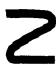
\includegraphics[keepaspectratio]{images/part001_ffa48347.jpg}}

注记. - 1) 当 \(\mathfrak{F}\) 是一个由非下半连续的函数 \(\geqslant 0\) 组成的不可数有向集时，关系式 (11) 不一定成立。例如取 \(X = R\) ，\(\mu\) 为 \(R\) 上的 Lebesgue 测度，并考虑按 \(\leqslant\) 有向的集 \(\mathfrak{F}\) ，它由所有特征函数 \(\varphi_{M}\) （ \(M\) 取遍 \(R\) 的有限子集）组成。这时 \(\mu^{*}(\varphi_{M}) = 0\) 对每个有限子集 \(M\) 成立，因为一点含于一个长度任意小的开区间中，从而由 No.~2 的定义 3 与命题 9，化为一点的集合的特征函数的上积分为零。但 \(\mathfrak{F}\) 的上包络是等于 1 的常值函数，而 \(\mu^{*}(1) = +\infty\) 。

\begin{enumerate}
\def\labelenumi{\arabic{enumi})}
\setcounter{enumi}{1}
\tightlist
\item
  注意，对递减序列 \((f_n)\) （诸函数 \(\geqslant 0\) ），不一定有 \(\mu^{*}(\inf_{n} f_n) = \inf_{n} \mu^{*}(f_n)\) ，即使 \(\mu^{*}(f_n) < +\infty\) 对所有 \(n\) 成立（参见 §4, 习题 8 c)）。
\end{enumerate}

命题 13. --- 对每个序列 \((f_n)\) （诸数值函数 \(\geqslant 0\) ，定义在 \(X\) 上），

\[
\mu^ {*} \left(\sum_ {n = 1} ^ {\infty} f _ {n}\right) \leqslant \sum_ {n = 1} ^ {\infty} \mu^ {*} (f _ {n}).\tag{12}
\]

只需对递增的函数序列 \(g_{n} = \sum_{k=1}^{n} f_{k}\) 应用关系式 (10)，并同时注意到由 (9) 有

\[
\mu^ {*} (g _ {n}) \leqslant \sum_ {k = 1} ^ {n} \mu^ {*} (f _ {k}).
\]

在 §5, No.~6 中，我们将给出使 (12) 的两端相等的条件。

命题 14（Fatou 引理）. --- 对每个序列 \((f_{n})\) （诸数值函数 \(\geqslant 0\) ），

\[
\mu^ {*} \left(\liminf _ {n \to \infty} f _ {n}\right) \leqslant \liminf _ {n \to \infty} \mu^ {*} (f _ {n})  .\tag{13}
\]

对每个整数 \(n\) ，令 \(g_{n} = \inf_{p\geqslant 0}f_{n + p}\) ；序列 \((g_n)\) 递增，且 \(\liminf_{n\to \infty}f_n = \sup_n g_n\) ，由此，由 (10) 得

\[
\mu^ {*} (\liminf _ {n \to \infty} f _ {n}) = \sup _ {n} \mu^ {*} (g _ {n});
\]

但由于 \(g_{n} \leqslant f_{n+p}\) 对 \(p \geqslant 0\) 成立，有 \(\mu^{*}(g_{n}) \leqslant \mu^{*}(f_{n+p})\) ，由此 \(\mu^{*}(g_{n}) \leqslant \inf_{p \geqslant 0} \mu^{*}(f_{n+p})\) ，最终得

\[
\mu^ {*} \left(\operatorname * {l i m i n f} _ {n \to \infty} f _ {n}\right) \leqslant \sup _ {n} \left(\inf _ {p \geqslant 0} \mu^ {*} (f _ {n + p})\right) = \operatorname * {l i m i n f} _ {n \to \infty} \mu^ {*} (f _ {n}).
\]

推论. --- 设 \((f_{n})\) 是数值函数 \(\geqslant0\) 的一个序列，使得对每个 \(x\in X\) ，\(\lim_{n\to\infty}f_{n}(x)=+\infty\) 。若 \(\mu\) 不是零测度，则 \(\lim_{n\to\infty}\mu^{*}(f_{n})=+\infty\) 。

若 \(f_{0}\) 是等于 \(+\infty\) 的常值函数，则 \(f_{0}\) 是 \(K_{+}\) 中所有函数的上包络，且由于 \(\mu \neq 0\) ，有 \(\mu^{*}(f_{0}) > 0\) ；但由于 \(f_{0} = \alpha f_{0}\) 对每个 \(\alpha > 0\) 成立，必然有 \(\mu^{*}(f_{0}) = +\infty\) （命题 11）。于是不等式 (13) 表明 \(\mu^{*}(f_{n})\) 随 n 趋于 \(+\infty\) 。

命题 15. --- 对每个标量 \(\alpha > 0\) 以及每一对正测度 \(\mu, \nu\) （在 \(X\) 上），

\[
(\alpha \mu) ^ {*} = \alpha \mu^ {*}\tag{14}
\]

\[
(\mu + \nu) ^ {*} = \mu^ {*} + \nu^ {*}\tag{15}
\]

此外，关系 \(\mu \leqslant \nu\) 蕴含 \(\mu^{*} \leqslant \nu^{*}\) 。

我们来证明关系式 (15)。令 \(\lambda = \mu + \nu\) ；于是 \(\lambda(f) = \mu(f) + \nu(f)\) 对 \(f \in \mathcal{K}_+\) 成立；对 \(f \in \mathcal{I}_+\) ，\(\lambda^*(f)\) （相应地 \(\mu^*(f), \nu^*(f)\) ）的值是 \(\lambda(g)\) （相应地 \(\mu(g), \nu(g)\) ）当 \(g\) 跑遍（按 \(\leqslant\) 有向的）所有 \(g \in \mathcal{K}_+\) （满足 \(g \leqslant f\) ）所成之集时的极限；因此 \(\lambda^*(f) = \mu^*(f) + \nu^*(f)\) 。最后，若 \(f\) 是定义在 X 上的任一函数 \(\geqslant 0\) ，则 \(\lambda^*(f)\) （相应地 \(\mu^*(f), \nu^*(f)\) ）是 \(\lambda^*(h)\) （相应地 \(\mu^*(h), \nu^*(h)\) ）当 \(h\) 跑遍（按 \(\geqslant\) 有向的）所有函数 \(h \in \mathcal{I}_+\) （满足 \(h \geqslant f\) ）所成之集时的极限；再次取极限，便得 \(\lambda^*(f) = \mu^*(f) + \nu^*(f)\) ，这就证明了 (15)。关系式 (14) 类似地建立。最后，若 \(\mu \leqslant \nu\) ，则可写 \(\nu = \mu + (\nu - \mu)\) ，其中 \(\nu - \mu \geqslant 0\) ，因此 \(\nu^* = \mu^* + (\nu - \mu)^*\) ，这表明 \(\mu^* \leqslant \nu^*\) 。

\subsection{任意集合的外测度}

定义 4. --- 设 \(\mu\) 是 X 上的正测度；对 X 的每个子集 A ，上积分 \(\mu^{*}(\varphi_{\mathrm{A}})\) 称为 A （关于测度 \(\mu\) ）的外测度，记作 \(\mu^{*}(\mathrm{A})\) 。

这样，一个集合的外测度是一个数 \(\geqslant0\) ，有限或等于 \(+\infty\) ，且对开集而言，它与 No.~2 的定义 2 中所定义的外测度一致。

命题 16. --- 若 A 与 B 是 X 的两个子集，满足 A ⊂ B，则 \(\mu^{*}(A) \leqslant \mu^{*}(B)\) 。

推论. --- X 中每个相对紧集的外测度都是有限的。

事实上，这样的集合含于一个相对紧的开集（GT, I, §9, No.~7, 命题 10），而后者的外测度是有限的（No.~2, 命题 5）。

命题 17. --- 若 \((\mathrm{A}_{n})\) 是 X 的子集的一个递增序列，则 \(\mu^{*}(\bigcup_{n}\mathrm{A}_{n})=\sup_{n}\mu^{*}(\mathrm{A}_{n})\) 。

命题 18. --- 对 X 的子集的每个序列 (A \(_{n}\) )，

\[
\mu^ {*} \left(\bigcup_ {n} \mathrm{A} _ {n}\right) \leqslant \sum_ {n} \mu^ {*} (\mathrm{A} _ {n}).
\]

这些命题就是 No.~3 的命题 10 与 13 以及定理 3 对集合的特征函数而言的翻译。

命题 19. --- 对 X 的每个子集 A ，\(\mu^{*}(A)\) 是包含 A 的诸开集的外测度的下确界。

若 \(\mu^{*}(\mathbf{A}) = +\infty\) ，命题是显然的。在相反的情形，对每个 \(\varepsilon\) （满足 \(0 < \varepsilon < 1\) ），存在函数 \(f \in \mathcal{I}_{+}\) 使 \(\varphi_{\mathrm{A}} \leqslant f\) 且 \(\mu^{*}(\mathrm{A}) \leqslant \mu^{*}(f) \leqslant \mu^{*}(\mathrm{A}) + \varepsilon\) 。设 \(\mathbf{G}\) 为诸 \(x \in \mathbf{X}\) （满足 \(f(x) > 1 - \varepsilon\) ）所成之集。由于 \(f\) 下半连续，\(\mathbf{G}\) 是开集（GT, IV, §6, No.~2, 命题 1）且包含 A；另一方面 \(f \geqslant (1 - \varepsilon)\varphi_{\mathrm{G}}\) ，由此

\[
\mu^ {*} (\mathrm{G}) \leqslant \frac {1}{1 - \varepsilon} \mu^ {*} (f) \leqslant \frac {1}{1 - \varepsilon} \left(\mu^ {*} (\mathrm{A}) + \varepsilon\right);
\]

由于 \(\varepsilon\) 任意，可见 \(\mu^{*}(\mathbf{G})\) 与 \(\mu^{*}(\mathbf{A})\) 可相差得任意小，由此得命题。

\section{可忽略函数与可忽略集}

\subsection{可忽略的正函数}

定义 1. --- 给定一个测度 \(\mu\) 于局部紧空间 \(X\) 上，数值函数 \(f \geqslant 0\) （有限或否，定义在 \(X\) 上）称为关于测度 \(\mu\) 可忽略的，如果 \(|\mu|^*(f) = 0\) 。

这时我们也称 f 是 \(\mu\) -可忽略的，或在不致混淆时简称可忽略的。

命题 1. --- 若 \(f\) 是一个可忽略的函数 \(\geqslant 0\) ，则每个数值函数 \(g\) （满足 \(0 \leqslant g \leqslant \alpha f\) ， \(\alpha\) 为标量 \(> 0\) ）都是可忽略的。

事实上，\(0 \leqslant |\mu|^*(g) \leqslant \alpha |\mu|^*(f) = 0\)

命题 2. --- 序列 \((f_{n})\) （诸函数为可忽略的 \(\geqslant0\) ）的和与上包络都是可忽略的。

事实上，\(|\mu|^*(\sum_n f_n) \leqslant \sum_n |\mu|^*(f_n) = 0\) （§1, No.~3, 命题 13），且 \(\sup_n f_n \leqslant \sum_n f_n\) 。

命题 3. --- 下半连续函数 \(f \geqslant 0\) （定义在 \(X\) 上）可忽略，必须且只须 \(f\) 在 \(\mu\) 的支集上为零。

若 \(|\mu|^*(f) = 0\) ，则 \(|\mu|(g) = 0\) 对每个函数 \(g \in \mathcal{H}_+\) （满足 \(g \leqslant f\) ）成立；由此（Ch. III, §2, No.~3, 命题 9）推出 \(g\) 在 \(\mu\) 的支集 S 上为零；由于 \(f\) 是诸函数 \(g \in \mathcal{H}_+\) （满足 \(g \leqslant f\) ）的上包络（§1, No.~1, 引理），故在 S 上 \(f(x) = 0\) 。反之，若在 S 上 \(f(x) = 0\) ，则在 S 上 \(g(x) = 0\) 对每个函数 \(g \in \mathcal{H}_+\) （满足 \(g \leqslant f\) ）成立，因此（Ch. III, §2, No.~3, 命题 8）\(|\mu|(g) = 0\) ，按定义这蕴含 \(|\mu|^*(f) = 0\) 。

\subsection{可忽略集}

定义 2. --- 给定一个测度 \(\mu\) 于局部紧空间 \(X\) 上，子集 \(A\) ⊂ \(X\) 称为关于测度 \(\mu\) 可忽略的，如果 \(|\mu|^*(A) = 0\) 。

我们也说 A 是 \(\mu\) -可忽略的，或在不致混淆时简称可忽略的。说特征函数 \(\varphi_{A}\) 可忽略是一回事。

命题 4. --- 可忽略集的每个子集都是可忽略的；可忽略集的可数并是可忽略的。

这是命题 1 与命题 2 的直接推论。

例子. --- 设 \(\mu\) 是 R 上的 Lebesgue 测度。每个化为一点的集合 \(\{x_{0}\}\) 都是可忽略的（参见 §1, No.~3, 注记 1）。由此推出 R 的每个可数子集关于 Lebesgue 测度都是可忽略的。该命题的逆命题不成立（§4, 习题 4 b)）。

命题 5. --- \(\mu\) 的支集 S 的余集是 X 中最大的可忽略开集。

事实上，由命题 3，要使开集 G 可忽略，必须且只须 \(G \cap S = \varnothing\) ，即 \(G \subset CS\) 。

\subsection{几乎处处成立的性质}

设 X 是局部紧空间，\(\mu\) 是 X 上的测度。若 \(P\{x\}\) 是一个性质，则性质 \(\langle P\{x\}\) 几乎处处（关于 \(\mu\) ）按定义等价于性质 \(\langle\) 由满足 \((x \in X \text{ 且不 } P\{x\})\) 的 x 所组成的集是 \(\mu\) -可忽略的。

定理 1. --- 要使定义在 X 上的数值函数（有限或否）\(f \geqslant 0\) 是可忽略的，必须且只须 \(f(x) = 0\) 几乎处处成立。

该条件是必要的。事实上，设 \(f\) 可忽略，并设 \(N\) 为诸 \(x \in X\) （满足 \(f(x) \neq 0\) ）所成之集；则 \(\varphi_N \leqslant \sup_n (nf)\) ，因此 \(\varphi_N\) 可忽略（No.~1, 命题 1 与 2）。

该条件是充分的。设使 \(f(x) \neq 0\) 的点所成的集 N 可忽略；则 \(f \leqslant \sup_{n} n\varphi_{N}\) ，因此 f 可忽略（No.~1, 命题 1 与 2）。

命题 6. --- 若 \(f\) 与 \(g\) 是两个函数 \(\geqslant 0\) （有限或否，定义在 X 上），使得 \(f(x) = g(x)\) 几乎处处成立，则 \(|\mu|^*(f) = |\mu|^*(g)\) 。

设 N 为诸点 \(x \in X\) （满足 \(f(x) \neq g(x)\) ）所成的可忽略集。由于函数 \(\inf(f, g)\) 与 \(\sup(f, g)\) 除去 N 的点外相等，只需在假设 \(f \leqslant g\) 下证明命题。设 h 为在 N 的点上等于 \(+\infty\) 、在 CN 上等于 0 的函数；则 \(f \leqslant g \leqslant f + h\) ，于是

\[
| \mu | ^ {*} (f) \leqslant | \mu | ^ {*} (g) \leqslant | \mu | ^ {*} (f + h) \leqslant | \mu | ^ {*} (f) + | \mu | ^ {*} (h) = | \mu | ^ {*} (f)
\]

（因为 \(h\) 可忽略），由此得命题。

命题 7. --- 若 \(f\) 是一个函数 \(\geqslant 0\) （定义在 \(X\) 上），满足 \(|\mu|^*(f) < +\infty\) ，则 \(f(x)\) 几乎处处有限。

事实上，设 N 为诸点 \(x \in X\) （满足 \(f(x) = +\infty\) ）所成之集；对每个整数 n，\(n\varphi_{N} \leqslant f\) ，由此 \(n|\mu|^{*}(\varphi_{N}) \leqslant |\mu|^{*}(f)\) ；由于 n 可任意大，\(|\mu|^{*}(N) = 0\) 。

然而，即使 X 是紧的，一个定义在 X 上且处处有限的函数 \(f \geqslant 0\) 也可能有无穷的上积分，例子是 X = {[}0, 1{]}，\(f(x) = 1/x\) （对 x \textgreater{} 0）且 \(f(0) = 0\) ，\(\mu\) 为 X 上的 Lebesgue 测度。

\subsection{等价函数类}

设 \(\mu\) 是局部紧空间 \(X\) 上的一个测度。给定一个集合 \(F\) ，两个映射 \(f, g\) （从 \(X\) 到 \(F\) 中）称为关于 \(\mu\) 等价的（或 \(\mu\) -等价的，或在不致混淆时简称等价的），如果 \(f(x) = g(x)\) 在 \(X\) 中几乎处处成立。由于两个可忽略集之并是可忽略的，这样确实在集 \(F^X\) —— 由 \(X\) 到 \(F\) 中的全体映射组成 —— 中定义了一个等价关系；当我们说到这样一个函数 \(f\) 的等价类（不加其他说明）时，指的将是与 \(f\) 几乎处处相等的全体函数所成的类；在本章及以后各章中，我们将用记号 \(\widetilde{f}\) 表示这个类。

命题 8. --- 设 \((\mathrm{F}_{n})\) 是集合的一个可数族（有限或无穷）。对每个指标 n，设 \(f_{n}, g_{n}\) 是从 X 到 \(F_{n}\) 中的两个等价映射；则存在一个可忽略集 H ，使得对每个 \(x \notin H\) ，对一切 n 有 \(f_{n}(x) = g_{n}(x)\) 。

事实上，集 \(H_{n}\) —— 由诸 \(x \in X\) （满足 \(f_{n}(x) \neq g_{n}(x)\) ）组成 —— 是可忽略的，因此它们的并 H 也可忽略（No.~2, 命题 4），而这个集满足要求。

推论. --- 若 \(\varphi\) 是从 \(\prod_{n} F_n\) 到集合 \(G\) 中的一个映射，则映射 \(\varphi((f_n))\) 与 \(\varphi((g_n))\) （从 \(X\) 到 \(G\) 中）是等价的。

我们用 \(\varphi((\widetilde{f}_n))\) 表示每个函数 \(\varphi((f_n))\) 的等价类，其中 \(f_n\) 是类 \(\widetilde{f}_n\) 中的任意函数。

特别地，若 F 是 R 上的向量空间，则定义 \(\widetilde{f} + \widetilde{g}\) 与 \(\alpha\widetilde{f}\) 分别为 \(f + g\) 与 \(\alpha f\) 的等价类（f 与 g 是从 X 到 F 中的映射，而 \(\alpha\) 为标量）；这样，我们在从 X 到 F 中的映射的等价类所成之集上得到一个向量空间结构：而且，这就是 \(F^{X}\) 的结构关于由满足 \(\widetilde{f} = \widetilde{0}\) 的映射 f 组成的线性子空间（即几乎处处为零的函数，我们也称之为（取值于 F 的）可忽略函数）的商空间结构。类似地定义乘积 \(\widetilde{g}\widetilde{f}\) ，其中 \(\widetilde{f}\) 是从 X 到 F 中的映射的一个等价类，而 \(\widetilde{g}\) 是定义在 X 上的（有限）数值函数的一个等价类：这样，从 X 到 F 中的映射的等价类所成之集就具有一个在定义于 X 上的有限数值函数的等价类所成之集（它自身具有一个环结构）上的模结构。若 F 是 R 上的代数，则类似地在从 X 到 F 中的映射的等价类所成之集上定义一个代数结构。

设 F 是可度量的拓扑空间，并考虑 F 上一个与其拓扑相容且由伪距离的可数族 \(\rho_{n}\) 定义的一致结构（GT, IX, §§1 与 2）；要使从 X 到 F 中的两个映射 f, g 等价，必须且只须数值函数 \(\rho_{n}(f,g)\) 都可忽略；事实上，这等价于说 X 中存在一个可忽略集 H ，使得对每个 \(x\notin H\) ，对一切 n 有 \(\rho_{n}(f(x),g(x))=0\) ，即 \(f(x)=g(x)\) 。特别地，若 F 是可度量的局部凸空间，且 \((q_{n})\) 是定义 F 的拓扑的可数半范数族（TVS, II, §4, No.~1），则要使从 X 到 F 中的两个映射 f, g 等价，必须且只须数值函数 \(q_{n}(\mathbf{f}(x)-\mathbf{g}(x))\) 都可忽略。

命题 9. --- 设 f 与 g 是从 X 到 Hausdorff 拓扑空间 F 中的两个连续映射；要使 f 与 g 等价，必须且只须 \(f(x) = g(x)\) 在 \(\mu\) 的支集的每点处成立。

事实上，由诸 \(x \in X\) （满足 \(f(x) \neq g(x)\) ）组成的集是一个开集（GT, I, §8, No.~1）；要使它可忽略，必须且只须它与 \(\mu\) 的支集不相交（No.~2, 命题 5）。

命题 10. --- 设 F 是 R 上的 Hausdorff 局部凸空间，使得在 F 的对偶 F' 中存在一个序列 ( \(a_{n}^{\prime}\) ) ，它在弱拓扑 \(\sigma(F^{\prime},F)\) 下稠密（TVS, II, §6, No.~2）。要使从 X 到 F 中的两个映射 f, g 等价，必须且只须对每个 n，数值函数 \(\langle\mathbf{f}(x),\mathbf{a}_{n}^{\prime}\rangle\) 与 \(\langle\mathbf{g}(x),\mathbf{a}_{n}^{\prime}\rangle\) 等价。

该条件显然是必要的。反之，若它被满足，则存在一个可忽略集 H ，使得对每个 \(x \notin H\) ，对一切 n 有 \(\langle \mathbf{f}(x), \mathbf{a}_{n}^{\prime} \rangle = \langle \mathbf{g}(x), \mathbf{a}_{n}^{\prime} \rangle\) ；这表明弱连续线性形式 \(\mathbf{z}^{\prime} \mapsto \langle \mathbf{f}(x), \mathbf{z}^{\prime} \rangle\) 与 \(\mathbf{z}^{\prime} \mapsto \langle \mathbf{g}(x), \mathbf{z}^{\prime} \rangle\) （在 \(F^{\prime}\) 上）在各点 \(a_{n}^{\prime}\) 处相等，从而由假设它们恒等，这就证明了 \(\mathbf{f}(x) = \mathbf{g}(x)\) 对所有 \(x \notin H\) 成立。

注意，命题 10 的假设特别适用于下述情形：F 是可度量且可分的 \(^{1}\) 局部凸空间（TVS, III, §3, No.~4, 命题 6 的推论 2）。

\subsection{几乎处处有定义的函数}

按照 No.~3 中的定义，从 X 的子集 A 到集合 F 中的映射 f 称为几乎处处有定义的，如果它在其上定义的集 A 的余集是可忽略集。我们仍称 f 的等价类（记作 \(\widetilde{f}\) ）为下述每个函数的等价类：该函数定义在整个 X 上，且在 f 有定义的点处等于 \(f(x)\) （诸点 \(x \in X\) ）；显然这个类只依赖于 f。~两个几乎处处有定义的函数 f, g 当 \(\widetilde{f} = \widetilde{g}\) 时仍称为等价的：这就是说，使 \(f(x)\) 与 \(g(x)\) 都有定义且相等的点所成的集具有可忽略的余集。

由此立即推出，No.~4 的命题 8 及其推论可以推广到下述情形：在其叙述中只假设每个函数 \(f_{n}, g_{n}\) 都几乎处处有定义；这时函数 \(\varphi((f_{n}))\)

和 \(\varphi((g_n))\) 本身也几乎处处有定义；\(\varphi((f_n))\) 的等价类仍是 \(\varphi((\widetilde{f}_n))\) 。

一个几乎处处有定义、取值于向量空间 F 中的函数，如果等价于 0，仍称为可忽略的。若 f 是取值于 F 中的可忽略函数，而 u 是从 F 到向量空间 G 中的线性映射，则复合函数 \(u \circ f\) （几乎处处有定义）是可忽略的；类似地，对每个几乎处处有定义的（有限）数值函数 g，函数 gf （几乎处处有定义）是可忽略的。

\pandocbounded{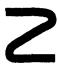
\includegraphics[keepaspectratio]{images/part001_e94daaaa.jpg}}

必须注意，在取值于 F 且几乎处处有定义的函数所成的集中，内合成法则 \((\mathbf{f},\mathbf{g})\mapsto\mathbf{f}+\mathbf{g}\) 不是群法则，因为虽然函数 0 确是此法则的中性元，但若 f 不是处处有定义，则不存在使 \(f+g=0\) 的函数 g。这正是引入等价类 \(\widetilde{f}\) 的动机，这些类确实构成一个向量空间。

设 \((f_n)\) 是映射到拓扑空间 F 中的一列映射，其中每个都在 X 中几乎处处有定义。我们说序列 \((f_n)\) 在 X 中几乎处处（逐点）收敛于 f，如果由下述点 \(x \in X\) 组成的集具有可忽略的余集：所有 \(f_n(x)\) 在该点有定义，且序列 \((f_n(x))\) 有等于 \(f(x)\) 的极限。显然，若对每个 n，函数 \(g_n\) （几乎处处有定义）等价于 \(f_n\) ，则序列 \((g_n)\) 也几乎处处收敛于 f。

若 F 是拓扑向量空间，则类似地定义一个几乎处处收敛的级数，其通项是在 X 中几乎处处有定义、取值于 F 中的函数 \(f_{n}\) ；这个级数的和是在部分和 \(\sum_{k=1}^{n}\mathbf{f}_{k}(x)\) 有定义且有极限的那些点处有定义的函数，其类只依赖于诸类 \(\widetilde{f}_{n}\) 。

\subsection{\texorpdfstring{取值于 \(\overline{R}\) 中的函数的等价类}{取值于 R-bar 中的函数的等价类}}

按照 No.~3 中的定义，我们说一个函数 \(f\) （在 \(X\) 中几乎处处有定义，取值于 \(\overline{\mathbf{R}}\) 中）几乎处处有限，如果由诸 \(x \in X\) （使 \(f(x)\) 有定义且有限）组成的集具有可忽略的余集。几乎处处有限的函数等价于一个处处有限的函数；因此可把它的类 \(\widetilde{f}\) 等同于定义在 \(X\) 上（或在 \(X\) 中几乎处处有定义）的有限数值函数的一个类。特别地，两个几乎处处有限的函数的类的和与积有定义，且这些类所成之集是 \(\mathbf{R}\) 上的一个代数。若 \((f_n)\) 是取值于 \(\overline{\mathbf{R}}\) 中、几乎处处有定义且有限的函数序列，则部分和 \(\sum_{k=1}^{n} f_k(x)\) 几乎处处有定义；若对几乎所有的 \(x \in X\) ，它们有极限 \(f(x)\) （在 \(\overline{R}\) 中），我们仍说以 \(f_{n}\) 为通项的级数几乎处处收敛，且 f 是该级数的和（注意 f 不一定几乎处处有限）。

若 \(f\) 与 \(g\) 是在 \(X\) 中几乎处处有定义且有限的两个数值函数，则 \(\widetilde{f} + \widetilde{g}\) （相应地 \(\widetilde{f}\widetilde{g}\) ）是每个等于 \(f(x) + g(x)\) （相应地 \(f(x)g(x)\) ）的函数的类（等式在使该表达式有意义的诸点 \(x \in X\) 处成立）。注意，\(f\) 与 \(g\) 可以都处处有定义，而 \(f(x) + g(x)\) （相应地 \(f(x)g(x)\) ）不对所有 \(x\) 有定义（GT, IV, §4, No.~3）；这时按定义 \(f + g\) （相应地 \(fg\) ）是在该表达式有定义的点处等于 \(f(x) + g(x)\) （相应地 \(f(x)g(x)\) ）的函数；因此它只是几乎处处有定义的。

设 \(f\) 与 \(g\) 是在 \(X\) 中几乎处处有定义的两个数值函数（有限或否），满足 \(f(x) \leqslant g(x)\) 几乎处处成立；若 \(f_1\) 等价于 \(f\) 且 \(g_1\) 等价于 \(g\) ，则显然 \(f_1(x) \leqslant g_1(x)\) 也几乎处处成立。因此所论关系只依赖于 \(f\) 与 \(g\) 的类；记作 \(\widetilde{f} \leqslant \widetilde{g}\) ，并且立即可以验证这个关系是取值于 \(\overline{\mathbf{R}}\) 中的函数的等价类所成之集上的一个序关系。若 \((\widetilde{f}_n)\) 是这样的一些类构成的可数族（有限或无穷），且对每个 \(n\) ，\(f_n\) 与 \(g_n\) 是两个几乎处处有定义、属于类 \(\widetilde{f}_n\) 的函数，则由 No.~4 的命题 8 推出，几乎处处有定义的函数 \(\sup_n f_n\) 与 \(\sup_n g_n\) 等价；因此它们的类只依赖于诸类 \(\widetilde{f}_n\) ，并且立即可验证它是这些类的上确界 \(\sup_n \widetilde{f}_n\) ——在按刚才所述方式排序的、取值于 \(\overline{\mathbf{R}}\) 中的函数的类所成之集中（从而这个集特别是一个格序集）。类似地可证明下确界 \(\inf_n \widetilde{f}_n\) 的存在性，并且有 \(\inf_n \widetilde{f}_n = -\sup_n (-\widetilde{f}_n)\) 。由此推出 \(\limsup_{n \to \infty} f_n\) 与 \(\limsup_{n \to \infty} g_n\) 也等价，它们的类记作 \(\limsup_{n \to \infty} \widetilde{f}_n\) ，等于 \(\inf_n (\sup_{p \geqslant 0} \widetilde{f}_{n+p})\) ；\(\liminf_{n \to \infty} \widetilde{f}_n\) 类似地定义。

数值函数 f（有限或否）如果等价于 0，就称为可忽略的；对于正的且处处有定义的函数，这个定义凭借定理 1 与定义 1 等价。要使 f 可忽略，必须且只须 \(|f|\) 可忽略（或 \(f^{+}\) 与 \(f^{-}\) 都可忽略）。

\section{\texorpdfstring{\(\mathrm{L}^{p}\) 空间}{L 的 p 次幂空间}}
